\documentclass[11pt,letterpaper,titlepage]{article}
% Change "article" to "report" to get rid of page number on title page
\usepackage{amsmath,amsfonts,amsthm,amssymb}
\usepackage[margin=1in]{geometry}
\usepackage{setspace}
\usepackage[T1]{fontenc}                                              %Provides T1 Font encoding for European characters
\usepackage{Tabbing}
\usepackage{array}                                                         % Allows for making new column types
\usepackage{dcolumn}					        % Provides decimal alignment column macros
\usepackage{fancyhdr}                                                  % Produce a "fancy" header using \rhead,\chead,\lhead
\usepackage{lastpage}
\usepackage{extramarks}
\usepackage{chngpage}
\usepackage{chngcntr} 						%figure and equation numbering by section
\usepackage{soul}
\usepackage{bookmark}                                                 % Prevents having to re-run due to labels
\usepackage[usenames,dvipsnames]{color}
\usepackage{graphicx,float,wrapfig}
%\usepackage{tocloft}							% Gives us the . . . in the TOC always and forever
\usepackage{ifthen}
\usepackage{listings}						% Allows for Listings
\usepackage{courier}                                                       % Provides the courier Font
\usepackage{subfig}
\usepackage{float}
%\usepackage[load-configurations = version-1]{siunitx}
\usepackage[arrowmos]{circuitikz}
%\usepackage{outlines}
\usepackage{pslatex}                                                    % This should switch the font to Times New Roman
%\usepackage[scaled=.92]{helvet}
\usepackage[printonlyused,withpage]{acronym}      % Creates acronym table of acronyms and definitions used
									        % in this document. \begin{acronym}[TDMA] ... \end{acronym}								   
\usepackage[final]{pdfpages}
%\usepackage{natbib}                                                   % Turn off for IEEE references
\usepackage{tikz-timing}
\usepackage{pdflscape}
\usepackage{multicol}
\usepackage{multirow}
\usepackage{wrapfig}
\usepackage{longtable}						% Provides the Longtable environment
\usepackage{colortbl}						% Provides \rowcolor{}
\usepackage[parfill]{parskip} 					% remove the dumb indents on all paragraphs
\usepackage[toc,page]{appendix}				% Provides more control over the Appendix
\usepackage{hyperref}						% Hyperlink output PDF Files
\usepackage[all]{hypcap}						% Fix the dumb hyperlink bug!!!

%\input{kvmacros}



%%%%%%%%%%%%%%%%%%%%%%%%%%%%%%%%%%%%%%%%%%%%%%%%
% TOC dots
%\renewcommand{\cftsecleader}{\cftdotfill{\cftdotsep}}
%%%%%%%%%%%%%%%%%%%%%%%%%%%%%%%%%%%%%%%%%%%%%%%%
% Setup the header and footer


\pagestyle{fancy}                                                       %
\fancyhead[L]{PICA LLC.}                                                 %
\fancyhead[R]{Business Plan}  %                                                   %
\fancyfoot[L]{\lastxmark}                                                      %                                                              %
\fancyfoot[C]{}
\fancyfoot[R]{Page\ \thepage\ of\ \pageref{LastPage}}                          %
\renewcommand\headrulewidth{0.4pt}                                      %
\renewcommand\footrulewidth{0.4pt}                                      %
%\renewcommand{\headheight}{14pt}
\headheight=14pt

\fancypagestyle{fancyplain}{
\fancyhead[L]{PICA LLC.}                                                 %
\fancyhead[R]{Business Plan}  %                                                 %
\fancyfoot[L]{}
\fancyfoot[C]{}                                                      %                                                              %
\fancyfoot[R]{}                          %
\renewcommand\headrulewidth{0.4pt}                                      %
\renewcommand\footrulewidth{0.4pt}                                      %
%\renewcommand{\headheight}{14pt}}
}
\definecolor{MyDarkGreen}{rgb}{0.0,0.4,0.0}
%%%%%%%%%%%%%%%%%%%%%%%%%%%%%%%%%%%%%%%%%%%%%%%%%
% Creating special column types -- mostly math types
%%%%%%%%%%%%%%%%%%%%%%%%%%%
% Start by defining some macros
\newcolumntype{d}[1]{D{.}{\cdot}{#1}}
\newcolumntype{.}{D{.}{.}{-1}}
\newcolumntype{,}{D{,}{,}{2}}
\newcolumntype{C}{>{$}c<{$}}
\newcolumntype{R}{>{$}r<{$}}
%%%%%%%%%%%%%%%%%%%%%%%%%%%%%%%%%%%%%%%%%%%%%%%%%
% For faster processing, load Matlab syntax for listings
\lstloadlanguages{MATLAB, [x86masm]Assembler, C++, VHDL}%
\lstset{frame=single,                                                                              % Single frame around code
        basicstyle=\tiny\ttfamily,             					   % Use small true type font
        keywordstyle=[1]\color{blue}\ttfamily,        				   % MATLAB functions bold and blue
        keywordstyle=[2]\color{purple},         				            % MATLAB function arguments purple
        keywordstyle=[3]\color{blue}\underbar,  			            % User functions underlined and blue
        identifierstyle=,                       						   % Nothing special about identifiers
                                                							   % Comments small dark green courier
        commentstyle=\usefont{T1}{pcr}{m}{sl}\color{MyDarkGreen}\scriptsize,
        stringstyle=\color{purple},             					   % Strings are purple
        showstringspaces=false,                 					   % Don't put marks in string spaces
        tabsize=5,                              						   % 5 spaces per tab
        %
        %%% Put standard MATLAB functions not included in the default
        %%% language here
        morekeywords={ra,stw, addi, ldw, bge, beq, br},
        %
        %%% Put MATLAB function parameters here
        morekeywords=[2]{on, off, interp},
        %
        %%% Put user defined functions here
        morekeywords=[3]{FindESS, homework_example},
        %
        morecomment=[l][\color{blue}]{...},     % Line continuation (...) like blue comment
        numbers=left,                           % Line numbers on left
        firstnumber=1,                          % Line numbers start with line 1
        numberstyle=\tiny\color{black},          % Line numbers are blue
        stepnumber=5,                            % Line numbers go in steps of 5
        breaklines=true,
        breakatwhitespace=false
        }  
 


% This is used to trace down (pin point) problems
% in latexing a document:
%\tracingall
\hfuzz4pt % I don't want to know about overfull hbox if < 2pt
%%%%%%%%%%%%%%%%%%%%%%%%%%%%%%%%%%%%%%%%%%%%%%%%%%%%%%%%%%%%%
% Some tools
\newcommand{\enterProblemHeader}[1]{\nobreak\extramarks{#1}{#1 continued on next page\ldots}\nobreak%
                                    \nobreak\extramarks{#1 (continued)}{#1 continued on next page\ldots}\nobreak}%
\newcommand{\exitProblemHeader}[1]{\nobreak\extramarks{#1 (continued)}{#1 continued on next page\ldots}\nobreak%
                                   \nobreak\extramarks{#1}{}\nobreak}%

\newlength{\labelLength}
\newcommand{\labelAnswer}[2]
  {\settowidth{\labelLength}{#1}%
   \addtolength{\labelLength}{0.25in}%
   \changetext{}{-\labelLength}{}{}{}%
   \noindent\fbox{\begin{minipage}[c]{\columnwidth}#2\end{minipage}}%
   \marginpar{\fbox{#1}}%

   % We put the blank space above in order to make sure this
   % \marginpar gets correctly placed.
   \changetext{}{+\labelLength}{}{}{}}%

\newcommand{\homeworkProblemName}{}%
\newcommand{\homeworkShortProblemName}{}
\newcounter{homeworkProblemCounter}%
\newenvironment{homeworkProblem}[2]
  {\stepcounter{homeworkProblemCounter}%
   \renewcommand{\homeworkProblemName}{#1}
   \renewcommand{\homeworkShortProblemName}{#2}
   \section*{\homeworkProblemName\ -- \homeworkShortProblemName}%
   \addcontentsline{toc}{section}{\homeworkShortProblemName}%
   \enterProblemHeader{\homeworkProblemName}}%
  {\exitProblemHeader{\homeworkProblemName}}%

\newcommand{\problemAnswer}[1]
  {\noindent\fbox{\begin{minipage}[c]{\columnwidth}#1\end{minipage}}}%

\newcommand{\problemLAnswer}[1]
  {\labelAnswer{\homeworkProblemName}{#1}}

\newcommand{\homeworkSectionName}{}%
\newlength{\homeworkSectionLabelLength}{}%
\newenvironment{homeworkSection}[1]%
  {% We put this space here to make sure we're not connected to the above.
   % Otherwise the changetext can do funny things to the other margin

   \renewcommand{\homeworkSectionName}{#1}%
   \settowidth{\homeworkSectionLabelLength}{\homeworkSectionName}%
   \addtolength{\homeworkSectionLabelLength}{0.25in}%
   \changetext{}{-\homeworkSectionLabelLength}{}{}{}%
   \subsection*{\homeworkSectionName}%
   \addcontentsline{toc}{subsection}{\homeworkSectionName}%
   \enterProblemHeader{\homeworkProblemName\ [\homeworkSectionName]}}%
  {\enterProblemHeader{\homeworkProblemName}%

   % We put the blank space above in order to make sure this margin
   % change doesn't happen too soon (otherwise \sectionAnswer's can
   % get ugly about their \marginpar placement.
   \changetext{}{+\homeworkSectionLabelLength}{}{}{}}%

\newcommand{\sectionAnswer}[1]
  {% We put this space here to make sure we're disconnected from the previous
   % passage

   \noindent\fbox{\begin{minipage}[c]{\columnwidth}#1\end{minipage}}%
   \enterProblemHeader{\homeworkProblemName}\exitProblemHeader{\homeworkProblemName}%
   \marginpar{\fbox{\homeworkSectionName}}%

   % We put the blank space above in order to make sure this
   % \marginpar gets correctly placed.
}%
   
\newcounter{subsubsubsection}[subsubsection]
\def\subsubsubsectionmark#1{}
\def\thesubsubsubsection {\thesubsubsection
     .\arabic{subsubsubsection}}
\def\subsubsubsection{\@startsection
     {subsubsubsection}{4}{\z@} {-3.25ex plus -1
     ex minus -.2ex}{1.5ex plus .2ex}{\normalsize\sf}}
% mj02r: original:
%\def\l@subsubsubsection{\@dottedtocline{4}
%     {4.8em}{4.2em}}
% mj02r: for VCE reports:
%\def\l@subsubsubsection{\@dottedtocline{4}
%     {7em}{3.8em}}
% mj02r, 29/12/2004: for thesis:
\def\l@subsubsubsection{\@dottedtocline{4}
     {11.1em}{4.6em}}

\makeatletter
\renewcommand{\paragraph}{\@startsection{paragraph}{4}{0ex}%
   {-3.25ex plus -1ex minus -0.2ex}%
   {1.5ex plus 0.2ex}%
   {\normalfont\normalsize\bfseries}}
\makeatother
   
% Includes a MATLAB script.
% The first parameter is the label, which also is the name of the script
%   without the .m.
% The second parameter is the optional caption.
\newcommand{\matlabscript}[2]
  {\begin{itemize}\item[]\lstinputlisting[language=MATLAB,caption=#2,label=#1]{#1.m}\end{itemize}}  
  
\newcommand{\ccode}[2]
  {\begin{itemize}\item[]\lstinputlisting[language={C++},caption=#2,label=#1]{#1.c}\end{itemize}}  
    
\newcommand{\assemblycode}[2]
  {\begin{itemize}\item[]\lstinputlisting[language={[x86masm]Assembler},caption=#2,label=#1]{#1.s}\end{itemize}}
  
 
\newcommand{\vhdlcode}[2]
  {\begin{itemize}\item[]\lstinputlisting[language={[AMS]VHDL},caption=#2,label=#1]{#1.vhd}\end{itemize}} 
  
\newcommand{\degree}{$^{\circ}$}
\renewcommand{\textbeta}{$\beta\ $}
\def\tm{\leavevmode\hbox{$\rm {}^{TM}$}}

%%%%%%%%%%%%%%%%%%%%%%%%%%%%%%%%%%%%%%%%%%%%%%%%%%%%%%%%%%%%%
%%%%%%%%%%%%%%%%%%%%%%%%%%%%%%%%%%%%%%%%%%%%%%%%
%This sets up the counters for the figures and equations to be numbered inside their sections
%\counterwithin{figure}{subsection}
%\counterwithin{equation}{section}
%\counterwithin{table}{subsection}
%\setcounter{secnumdepth}{5}
%\counterwithin{lst}{homeworkProblemCounter}
%%%%%%%%%%%%%%%%%%%%%%%%%%%%%%%%%%%%%%%%%%%%%%%%

%%%%%%%%%%%%%%%%%%%%%%%%%%%%%%%%%%%%%%%%%%%%%%%%%%%%%%%%%%%%%
% Make title
%\title{\vspace{2in}\textmd{\textbf{\hmwkAuthorName}}\\\normalsize\vspace{0.1in}\hmwkClass:\ \hmwkTitle \vspace{0.1in}\\Due\ on\ \hmwkDueDate\\\vspace{0.1in}\large{\textit{\hmwkClassInstructor\ \hmwkClassTime}}\vspace{3in}}
%\date{}
%\author{}
%\title{\vspace{2in}\textmd{\textbf{\hmwkClass:\ \hmwkTitle}}\\\normalsize\vspace{0.1in}\small{Due\ on\ \hmwkDueDate}\\\vspace{0.1in}\large{\textit{\hmwkClassInstructor\ \hmwkClassTime}}\vspace{3in}}
%\date{}
%\author{\textbf{\hmwkAuthorName}}

% IEEE Title
\title{Team PICA Business Plan}
\date{\today}
\author{Amy Ball, Nate Jen, Avery Sterk, Kendrick Wiersma}

%%%%%%%%%%%%%%%%%%%%%%%%%%%%%%%%%%%%%%%%%%%%%%%%%%%%%%%%%%%%%
% PDF Metadata
%\hypersetup{pdfinfo={
%                     Title={Team 01: Business Plan},
%                     Subject={Business 357},
%                     }}
%%%%%%%%%%%%%%%%%%%%%%%%%%%%%%%%%%%%%%%%%%%%%%%%%%%%%%%%%%%%%

\raggedright
\setcounter{tocdepth}{4}
\addtocontents{toc}{\protect\pagestyle{fancyplain}}
\addtocontents{lof}{\protect\pagestyle{fancyplain}}
\addtocontents{lot}{\protect\pagestyle{fancyplain}}
%\addtocontents{lol}{\protect\pagestyle{fancyplain}}

\begin{document}


%\maketitle % change this to a REAL titlepage
\begin{titlepage}
\begin{center}

\includegraphics[width=5in]{figures/TeamPicaLogo}

{\LARGE \textbf{P}ower \textbf{I}nformation \textbf{C}ollection \textbf{A}rchitecture}

\vspace{0.5in}

{\LARGE Business Plan}
\vspace{1in}

{\Large Engineering 340}

{\Large 2 March 2011}

{\Large Team 01: A. Ball, K. Wiersma, N. Jen, A. Sterk}

\vspace{1in}

\includegraphics[width=3in]{figures/Calvin_Logo}

\end{center}
\end{titlepage}
\newpage
\begin{abstract}
%The proposed business plan follows the development a power-monitoring system capable of monitoring total and circuit-by-circuit power usage for a given installation. Such a system would use non-invasive load monitoring techniques to monitor the flow of current through the feeder lines; the system can then aggregate all of this data, and perform data analysis to determine kilowatt hours used, reactive power, line frequency, and in some cases power factor. The system then can display this data to a user in real-time over a wall-mounted display unit or a web interface.

%The following report outlines the design of this system and the major decisions that the design team made. The major accomplishments thus far have been: Meeting with Consumer's Energy, Product competition research, defining a budget and per-system cost estimates, selecting features for inclusion, establishing rough requirements, investigating design possibilities, selecting a metering device for prototyping, and identifying unforeseen constraints. The remaining work for this project includes: solid-state breaker and monitor/controller design and implementation, base station design and implementation, E-meter design and implementation, component and system testing, and prototype construction.

%The final result of the project will be a working prototype which demonstrates the ability to correctly and accurately monitor power consumption. The project is scheduled to be completed by May 7, 2011.

This business plan describes the formation and operation of PICA, LLC., a company formed around the products designed by Team PICA as a senior design project at Calvin College. The company proposes to design, produce, and distribute power-monitoring equipment that may replace typical components of modern electrical building infrastructure. In particular, PICA, LLC.\ will produce a smart power meter for power companies to install on their customers' buildings and with which much more information regarding power quality can be measured, ``smart'' solid-state circuit breakers that improve user safety and deliver information about how much power each circuit in the building uses, and a base station to collect, archive, and display these measurements in real time. Armed with this much information, power consumers will be able to make wiser decisions regarding their power usage.

The market for ``smarter'' electronics and power monitoring continues to grow, and smart meters are already entering deployment on houses in select parts of the country. PICA, LLC.\ intends to produce devices that gather more information and collect and display it in a user-friendly style. The design team believes that these products are completely possible to make and distribute, and can be designed using the knowledge of electrical engineering and systems gained from Calvin's engineering program.

The team estimates first-year costs close to \$300 million, financed 60-40 from debt and equity. This means that about \$120 million will come from investors. The estimated payout time will be 5 years, by which time production and distribution means will be established and enacted.

\end{abstract}
%\setcounter{page}{0}
\tableofcontents
\thispagestyle{fancyplain}
\newpage
\thispagestyle{fancyplain}
\listoffigures
\listoftables
%\lstlistoflistings
\newpage

\protect\pagestyle{fancy}
\begin{spacing}{1.5}

%%%%%%%%%%%%%%%%%%%%%%%%%%%%%%%
% PPFS Stuff we don't use
%%%%%%%%%%%%%%%%%%%%%%%%%%%%%%%
%
%\section{Project Introduction}
\subsection{Overview of the Problem}
Standard electric meters were developed decades ago and are still used today, despite many technological advances in the last several years. Along with these technological advances, Americans have become accustomed to having access to large amounts of data, but due to the nature of the standard electric meter, data regarding the usage of power is severely limited. For the power companies, data from the meters is minimal and grid control is limited to manual operation, costing them time and money.
As the cost of electricity becomes higher and higher, electricity use in buildings is becoming a bigger concern and people have few cheap or simple ways to monitor this. Of the options available, most only address part of the whole problem, giving some information to the consumer and none to the power company or vice-versa. While there are devices such as breakers and fuses that provide electrical safety for buildings, advances in technology have made it possible to further improve safety but have not been implemented in a cost-effective way or made easily available to an average consumer, which for the purpose of this project shall be defined as a person without a mathematical or scientific education beyond high-school.

\subsection{Why the Project was Chosen}
Our team chose the project for several reasons; as future homeowners, the team has an interest in knowing more about power usage within a home. There are also many more people who would benefit from more accurate and useful data about power usage.

As good stewards of Earth we want to make sure the natural resources available are not wasted, and we believe that if there is access to more and better information, people will have a better opportunity to manage those resources more effectively. In addition, providing better information and control to the power companies can lead to less wasting of electricity on the provider's end, further contributing towards better use of Earth's resources.

Electricity-related deaths and injuries have been reduced due to devices such as fuses and breakers, but many still happen every year. As fellow human beings, we care and would like to minimize these incidents further. The technology is available and will benefit many people when implemented.

\subsection{Team Information}

Team 01, Team PICA seen in figure \ref{fig:teamphoto} consists of four engineers in Calvin College's Electrical and Computer Engineering concentration: Amy Ball, Nathan Jen, Avery Sterk, and Kendrick Wiersma.

\begin{figure}[htbp]
\begin{center}
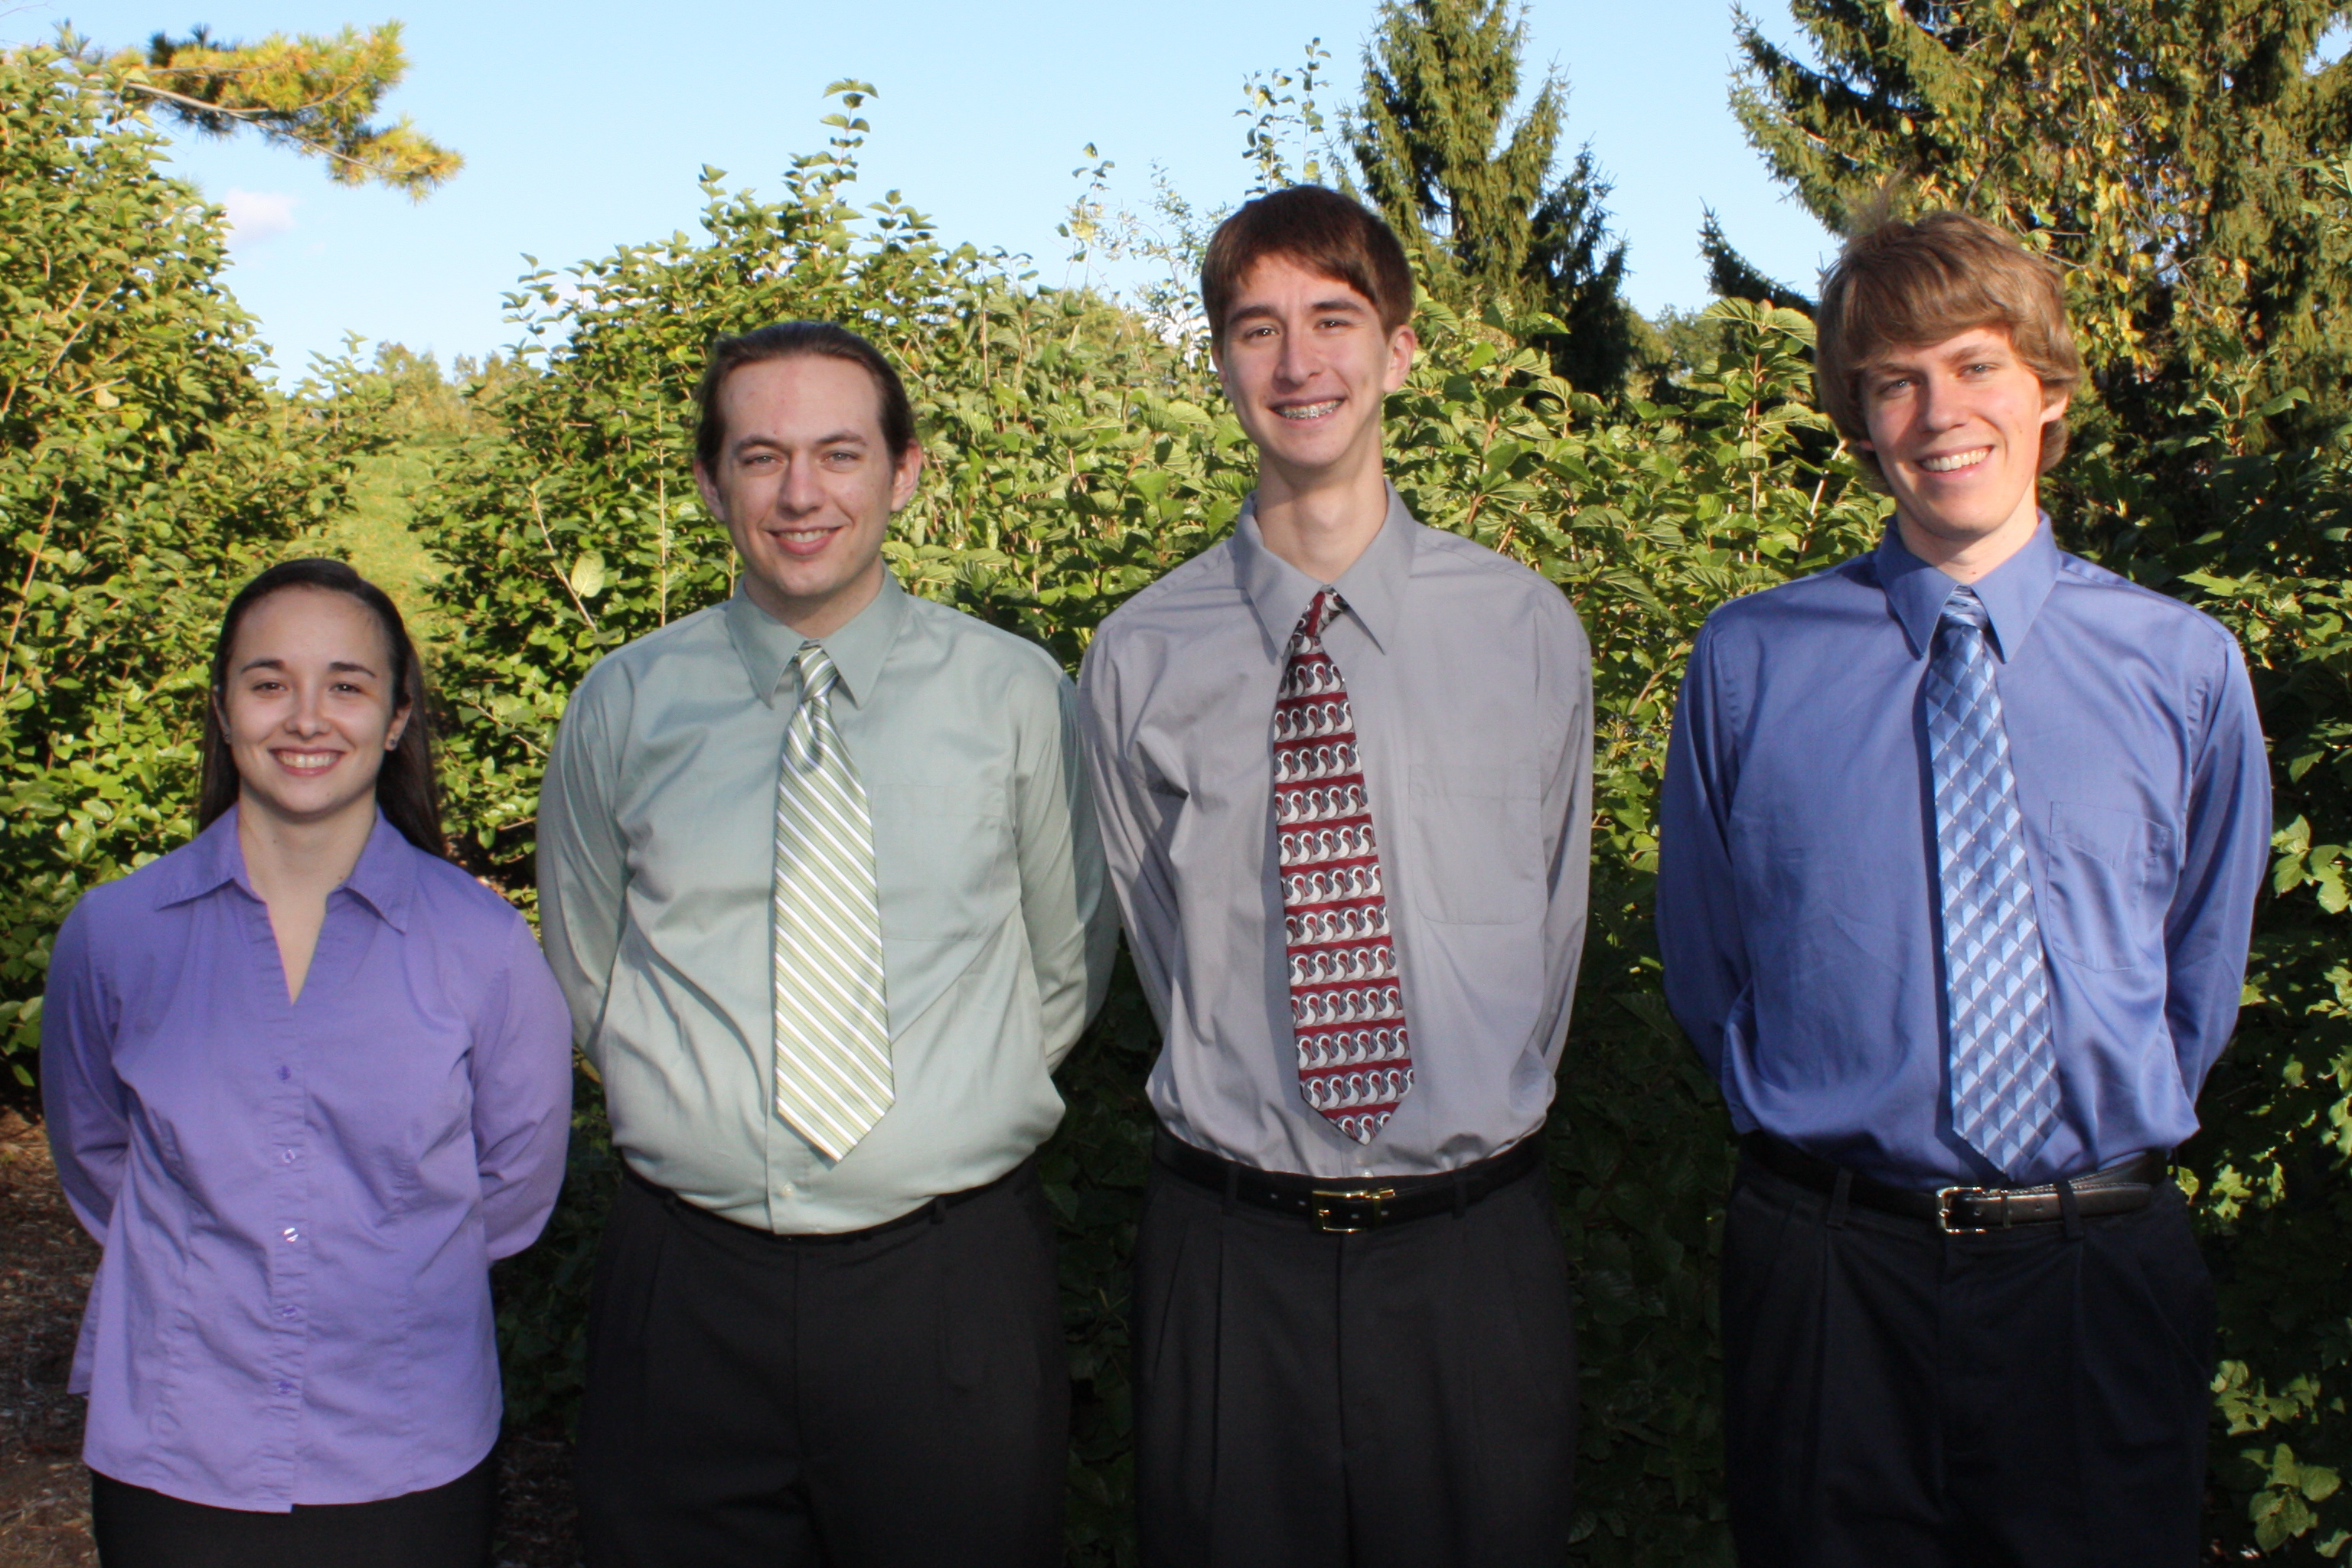
\includegraphics[width=6in]{figures/IMG_0865}
\caption{Team PICA, left to right: Amy Ball, Kendrick Wiersma, Nate Jen, and Avery Sterk.}
\label{fig:teamphoto}
\end{center}
\end{figure}

Amy works as an intern at Johnson Controls, where she works as part of the Systems Engineering Team. She brings good communication skills, circuit-building experience, and presentation skills to the project. Her section of the project is the solid-state breakers, especially working closely with much of the analog hardware involved with the project.

Kendrick works as an intern at Raytheon Missile Systems in the Electronics Center, where he performs embedded system design and verification. Kendrick hails from Tucson, Arizona where he was born and raised. He brings real-world project experience and experience working with embedded hardware and software to the team. Kendrick leads the development of the E-meter, which measures whole-building power consumption, reporting data to the power company and the PICA base station.

Nathan has worked at Amway on the production floor and has gained involvement with club leadership at Calvin College. He brings leadership experience and a good understanding of how smaller elements of a system fit together as a whole. His section of the project is the monitoring of individual circuits and some of the control logic for the breakers.

Avery worked as an intern at the SLAC National Accelerator Laboratory doing \ac{CAD} design. He brings varied experience with software design and implementation to the project. His section of the project is the base station, especially providing the primary user interface and designing embedded software.


%\include{overview}
%\include{requirements}
%\include{designGoals}
%\include{systemDesign}
%\include{majorDesignDecisions}
%\include{eMeterDesignAlt}
%\include{breakerMonitorDesignAlt}
%\include{ssbDesignAlt}
%\include{baseStationDesignAlt}
%\include{verification}

%%%%%%%%%%%%%%%%%%%%%%%%%%%%%%%%%
% What we'll use: make sure it's all uncommented in final
%%%%%%%%%%%%%%%%%%%%%%%%%%%%%%%%%
%
\section{Mission and Vision}

\subsection{Mission}
PICA LLC seeks to help our clients better understand how their home or business consumes power through the transparent application of technology in a culturally appropriate manner. We seek to develop cost effective solutions that exhibit quality worksmanship using our expertise in Electrical and Computer Engineering.

\subsection{Vision}
PICA LLC seeks to help in building a future where power consumption is an active choice. By using modern technology to enhance power metering, we believe that a future with less dependence on fossil fuels comes one step closer to reality.

\section{Industry Profile}
\subsection{Overview of the Problem}
Standard electric meters were developed decades ago and are still used today, despite many technological advances in the last several years. Along with these technological advances, Americans have become accustomed to having access to large amounts of data, but due to the nature of the standard electric meter, data regarding the usage of power is severely limited. For the power companies, data from the meters is minimal and grid control is limited to manual operation, costing them time and money.
As the cost of electricity becomes higher and higher, electricity use in buildings is becoming a bigger concern and people have few cheap or simple ways to monitor this. Of the options available, most only address part of the whole problem, giving some information to the consumer and none to the power company or vice-versa. While there are devices such as breakers and fuses that provide electrical safety for buildings, advances in technology have made it possible to further improve safety but have not been implemented in a cost-effective way or made easily available to an average consumer, which for the purpose of this project shall be defined as a person without a mathematical or scientific education beyond high-school.

\subsection{Major Customer Groups}
The two main customers of the PICA system are power companies and power consumers. The E-meter subsystem will only be sold to power companies, as they must in turn provide metering equipement to their customers. The base station and solid-state breakers will be sold to power consumers who are interested in knowing how much power they use in different regions of their buildings.

\subsection{Regulatory Requirements} % This has been fixed
The PICA system must meet certain codes in order to be safe enough for the customer to use, which will also protect from unexpected lawsuits. \ac{UL} is an independent product safety certification organization, which offers safety certifications to products \cite{UL_Web}. In order to gain the confidence of customers, the devices of the PICA system will be UL certifiable. The specific qualifications of \ac{UL} certification remain unknown to the design team, as the documents regarding the certification requirements are not publicly available. The system will also restrict \ac{EM} radiation to comply with \ac{FCC} Title 47 Part 15. It will also comply with \ac{ANSI} C12.19 and \ac{ANSI} C12.21 standards.

While these standards should ensure the general safety of the PICA devices, defects or unforeseen circumstances could imperil users or their property. The PICA system will provide a limited warranty against defects, but cannot be expected to foresee all possible circumstances. To this end, the devices will ship and work with a disclaimer regarding safe operating conditions and the hazards of tampering with the device.

In addition to ensuring the physical safety of the users, the system should also ensure the privacy and security of the users' information. While any wireless link runs the risk of packet interception and capture by a malicious observer, this will only affect the data currently being transferred, and data encryption schemes may greatly hinder these intrusions. The stored data will likely not be encrypted, but will not be actively transmitted: the only means of accessing this data will be through the software controls set in place by the base station or by physically removing the storage medium and removing the data from it. The base station software will use permissions-based file system access and will require a user to authenticate as an administrator before accessing this information. In this way, the user's data will be stored with access controls and will be kept private.

\subsection{Significant Trends and Growth Rate}
Recently, the demand for ``smarter'' and more informative devices has been increasing with the awareness of resource stewardship and the effects of human activity on the environment. Currently, power companies are investigating smart meters and deploying them to their customers in pilot programs. Power consumers are becoming more energy- and economically-aware, so the time is ripe for providing the products that PICA, LLC.\ proposes.

\subsection{Barriers to Entry and Exit}
The major barriers to entry is customer recognition. Although power companies may still be testing smart meters before deploying them to their customers, introducing them to a new product might be difficult if they are already near to making a decision. Additionally, power consumers will not be able to buy from PICA, LLC.\ unless they specifically know of it already.


%% echos will appear here



\section{Business Strategy}
\subsection{Desired image and position in market}
PICA seeks to be known as a leader in making consumers energy aware. This primarily means providing relevant information in an easy-to-understand format that allows users to make informed decisions about their energy usage. Our position in the market will likely be a part of the ``green'' market, which has been rapidly growing. However, we would like to aim for the consumer oriented part of this market, rather than reaching out to the part of the market dealing with clean power generation.
%\subsection{Company goals and objectives}
%\subsubsection{Operational}
%An operational goal is to retain a company structure that allows for rapid expansion, possibly including other national markets.
%\subsubsection{Financial}
%One finance related goal of PICA is to be successful enough that the company can start to address the objectives stated above.
%\subsubsection{Other}
%One big goal the business hopes to address is the gap between the electrical consumer and provider by producing products that meet both the needs of the power companies and homeowners. 
\subsection{SWOT analysis}
\subsubsection{Strengths}
One big strength of the product is that in a single system it addresses problems that previously would require multiple, independent systems and products. Another strength is the solid state breakers, which in addition to providing usage information also have a faster response time and include a safe automatic reset option.
\subsubsection{Weaknesses}
The biggest weakness is the cost of the system. While users want to know the information provided, many are not willing to pay a lot for that information. 
\subsubsection{Opportunities}
The idea of solid state breakers for home usage is relatively new and has not been taken advantage of, so there is a lot of potential growth in that area.
\subsubsection{Threats}
A big threat is that other companies have already started to establish themselves in similar fields. The PICA system may not provide enough of an advantage over these systems to be successful in an area where consumers have started to use these other systems.
\subsection{Competitive strategy}
%\subsubsection{Cost leadership}
As there is a high cost associated with the PICA products, the company will rely less on cost to remain competitive than on the differentiation and focus of the company. 
%\subsubsection{Differentiation}
The company has already started to differentiate itself primarily through the development of the solid state breakers. The company is also different from many in how we provide solutions to more than one problem the consumer and power company may have.
%\subsubsection{Focus}
The company hopes to remain competitive by continuing to focus on more aspects of the problems associated with power usage than potential competitors do. Instead of providing a solution relating only to single outlet usage, PICA will provide devices that can all work together, leaving room for easy expansion when the customer decides they want even more information.
%\include{products_services} % I assume we've already provided this?
\subsection{Target Market Definition} % Fixed
The target market for the entire PICA system comprises both electricity producers and electricity consumers, as set forth by the nature of the subsystems. As the power companies supply and own the electricity meters attached to the buildings to which they supply power, the PICA E-meter appeals only to the market of electricity-producing companies. The other two subsystems, the solid-state breakers and base station, target the power-consuming audience, as the devices will assist in monitoring power flow inside the building, where the power company has no presence. As these two markets are essentially exclusive in both membership and interest in the PICA subsystems, the E-meter will be able to function independently of the other consumer-targeted subsystems, and vice versa.

\subsubsection{Power Companies} % Fixed
As power companies currently distribute the whole-building metering hardware that determines how much energy their customer used, the E-meter clearly targets power companies. In fact, the power companies own the power-measuring hardware external to the buildings to while they provide power, so only they may replace or upgrade those devices. At present, power companies send trained meter-readers to read the data from most traditional power meters under their control. The PICA E-meter subsystem aims to improve on this process by automatically sending the measurements to the power company using a means and protocol selected by the particular company. While this will require some hardware customization for each company, the volume of company-specific production should allow the cost to develop the design to spread into a small per-unit cost.

The PICA E-meter subsystem also provides numerous more measures of power than the simple spinning-dial meters. For example, the E-meter will measure the frequency and the RMS voltage of the incoming supply lines, which help indicate the overall quality of power delivered to the customers in the area. This information may also help diagnose any observed issues with power delivery without dispatching a worker to take measurements by hand. In this way, power companies using the PICA E-meter can improve the quality of the service they provide and can save on the labor costs associated with making a site visit.

\subsubsection{Power Consumers}
Although the power company's customers cannot modify the metering panel installed by the power company, they are free to modify the other power distribution components inside their own buildings. The solid-state breakers fall into this category, and provide previously unavailable measurements regarding power consumption and its location within the building. However, as these breakers will replace the pre-existing breakers inside the building, the consumer must be convinced that using the PICA system is worth the trouble and cost of replacing the mechanical circuit breakers with the more feature-rich PICA breakers. To this effect, the most receptive market for the solid-state breakers includes homeowners and building managers who are curious or concerned about power usage inside their building. That is, the people for whom this information can inspire a meaningful change in practice will likely become the first adopters of the subsystem.

The product may also gain a following as an alternative to mechanical breakers in during the construction of a new home or building. This would likely require that the product already have a proven history of reliability and safety, so the previous group of cost- or environmentally-concerned individuals might have to adopt the produce first. If the PICA solid-state breakers become an alternative during construction, the net cost to the user will be lessened, as the building-to-be will not have any pre-existing breakers to discard or replace.

The base station may apply to either of these two consumer groups, as its primary purpose is to manage and interface with the other systems. It does not specifically require the solid-state breakers or the E-meter, but provides little value in a building without any installed PICA systems. The base station exists solely to manage and collect data from other PICA subsystems, as well as format and display these measurements, so its target audience consists of power consumers whose buildings contain at least one of the E-meter or solid-state breakers.

\subsubsection{Market Coordination}
As the E-meter subsystem caters exclusively to power companies while the other subsystems target power consumers, the complete PICA system has no clearly-defined market; neither of the two markets involved desires the entire system. Despite this separation, a clever marketing strategy could motivate one market to pressure the other.

In one scenario, a power company installs the PICA E-meter onto a select set of their customers' buildings. On its own, this should be a transparent change to the consumer. However, marketing the base station as a way to ``see what the power company sees'' about the power delivered could motivate some of the power-consuming market to purchase a PICA subsystem. Giving the power-consuming market a feeling of empowerment or equality to the power company could therefore motivate more consumer-side subsystem sales.

Conversely, the interests of the power-consuming market could generate interest from the power-producing market. In particular, a consumer who already owns the PICA solid-state breakers may appeal to the power company to provide the PICA E-meter: it would expand the amount of information available and give an accurate sense for the upcoming utility bill. Even without any PICA subsystems, the consumer could prod the power company for a PICA E-meter because it would give the power company more information on power quality, which could in turn increase the quality of service provided to the consumer. In these scenarios, the desires of the power-consumer market could influence demand in the power-producing market.

\subsection{Target Market Research} % Fixed
From the team's visit to Consumer's Energy in Jackson Michigan, power companies are very interested in smart home energy meters, such as PICA provides with the E-meter. The team presented a features list to the representative present. who affirmed that the features now included in the E-meter will be valuable to the power companies. However, power companies are already researching and testing smart meter prototypes and samples, so the E-meter will arrive fairly late relative to its competition. Still, of the thousands of power companies in the United States\cite{EIA_Intro}, the PICA system will surely prove interesting to others who may not have considered alternatives. Fewer than half of the homes expected to receive the smart-meter conversion have been converted to date, so the E-meter is still viable in the power company market\cite{Gtech_Smart_Meters}.

The remainder of the system, the base station and the solid-state breakers, will compete in a market of power consumers. The devices currently face a  market of 6,400,000 customers, according to an estimate from the project's Business 396 companion team. Of these customers, approximately 0.02\% may be interested in PICA, giving 12800 expected sales\cite{Gtech_Renew} given that we are a start up company. Additionally, despite the recent economic downturn, housing spending has experienced an upward trend\cite{Economic_Predictions}, which may indicate a possible increase in the number of houses that could be constructed with the PICA solid-state breaker technology. The market for the consumer-oriented subsystems seems to be healthy, and even growing, despite the recent economic slump.

%\subsubsection{Market Feasibility} % This has been fixed
In order for any product to succeed commercially, its perceived value must meet or exceed the price the customer would pay for it. If the PICA system as a whole is to be a feasible market success, it must surpass its competitors in providing value per price. From a practical standpoint, this involves either selling a comparable product for a lower price than the competition, or producing a superior product at a similar price. The PICA project generally aims to follow the second of these two paths. The solid-state circuit breakers include solid-station circuit breakers and circuit-by-circuit power monitoring, both of which seem to be unusual or even unique features, which in turn means that its feasibility depends on the value of its features rather than a lower price. The base station may be viewed as an accessory to the other subsystems, but its function as the output of the collected information gives it a very high value to anyone who desires the information collected by the other PICA devices, so its feasibility relies on its high perceived value, rather than on undercutting competition. The smart-metering aspects of the E-meter essentially meet the expectations set by other smart meters, so the market feasibility of the E-meter device depends more on the price than on the features, but its ties with the base station can provide additional feature value as well. Overall, the subsystems of the PICA project tend to focus on providing valuable features, rather than on reducing the price below that of the competitors.

\subsection{Consumer Cost Recovery} % this is already fixed
In 2009, the residential monthly electricity bill in the United States averaged to \$104.52\cite{DOE-EIA}. If the PICA base station and solid-state breakers sell with a retail price around \$400, then the investment will amount to approximately four months of electricity bills. If, as is intended, the PICA system allows users to more wisely manage their consumption habits, then homeowners who have purchased the base station and have either the solid-state breakers or the E-meter installed at their house should experience a decrease in their monthly bill, which could recover the initial cost of the system installation. A table summarizing the different savings and payback periods appears as table \ref{tab:cost-recoup}.

\begin{table}[htbp]
 \caption{Table of Cost Recovery Rates} \label{tab:cost-recoup}
 \begin{center}
 \begin{tabular}{|c|c|c|} \hline
 \rowcolor{lightgray}
 Relative Billing Reduced & Average Monthly Savings (\$) & Months to Recover \$400 \\ \hline
 0\% & 0 & - \\ \hline
 0.5\% & 0.52 & 765 \\ \hline
 1\% & 1.05 & 382 \\ \hline
 2\% & 2.09 & 192 \\ \hline
 3\% & 3.14 & 128 \\ \hline
 5\% & 5.23 & 77 \\ \hline
 10\% & 10.45 & 38 \\ \hline
 20\% & 20.90 & 19 \\ \hline
 \end{tabular}
 \end{center}
\end{table}

 As cost reduction rates depend entirely upon the user's response to the information, the recovery period for any given customer cannot be predicted. While reduction rates of $20\%$ and higher may be realized for some individuals, a savings rate of 3\% may be somewhat more typical. Using the \ac{DOE}'s monthly average of 908 kWh consumed per residence, this represents a decrease in average consumption of about 27 kWh per month per household. This amounts to 113 watts saved for eight hours for each of thirty days per month, equivalent to slightly more than one typical incandescent lightbulb. Such a reduction yields a payback period of 128 months, or slightly less than eleven years. If, however, the system could reduce consumption by twice this amount, the payback period would halve to just over five years, or 64 months.


\section{Parts and Project Costs}
\label{sec:parts_and_costs}

The project costs can be broken into fixed and variable costs, where fixed costs represent the costs the team will incur during the year and production start-up costs, while variable costs represent the long-term costs associated with production.

\subsection{Fixed Costs}
\subsubsection{Prototype parts}
Through the Senior Design class, the Calvin College Engineering department provided \$750 for prototype parts. Since the project has a large scope, the team needs to minimize the cost of any single part to stay within the given budget. As such, the team chose several parts more because of their low cost rather than for functionality. As such, the team sought donations and free samples whenever possible, including the TI MSP430 development kit from Texas Instruments and the ADE7763 power monitoring chips from Analog Devices. The team also obtained a pre-purchased Xilinx Virtex-5 development board. Table \ref{tab:proto_part_cost} shows the part donations and to-date purchases. 

\begin{table}[htdp]
\caption{Prototype part costs.}
\begin{center}
\begin{tabular}{|c|c|c|c|c|c|}\hline\rowcolor{lightgray}
Date & Item & Price & Quantity & Total & Running Total\\\hline
12-Sept & ADE7763 Samples & \$0.00 & 2 & \$0.00 & \$0.00\\\hline
15-Oct & SSOP to DIP Adapter 20-Pin & \$3.95 & 2 & \$7.90 & \$7.90\\\hline
15-Oct & Break Away Headers -- Straight	& \$2.50 & 1 & \$2.50 & \$10.40\\\hline
3-Nov  & TRANSF CURRENT .50" OPENING PCB & \$14.25 & 2 & \$28.50 & \$38.90\\\hline
15-Nov & TI Donation MSP430 & \$0.00 & 1 & \$0.00 & \$38.90\\\hline
02-Feb & XO Oscillators DIP-14 3.579545M & \$1.87 \ 2 \ \$3.74 \ \$42.64 \\\hline
02-Feb & Solid State Relay 25A & \$24.07 \ 2 \ \$48.14 \ \$90.78 \\\hline
02-Feb & LCD Graphic Display Modules & \$18.55 \ 1 \ \$18.55 \ \$109.33 \\\hline
02-Feb & FFC/FPC Connectors 0.5mm & \$1.29 \ 2 \ \$2.58 \ \$111.91 \\\hline
02-Feb & Headers and Wire Housings & \$1.13 \ 2 \ \$2.26 \ \$114.17 \\\hline
02-Feb & Synchro Chron LCD and Backlight & \$22.75 \ 1 \ \$22.75 \ \$136.92 \\\hline
\end{tabular}
\end{center}
\label{tab:proto_part_cost}
\end{table}%

\subsubsection{Labor}
Throughout the semester, the team has kept a log of how many hours they worked. Determining the cost of labor for the past semester based on these records, the team can also more accurately forecast the labor cost for next semester. So far, the team has logged 348 hours, with another 40 estimated before the end of the semester. Extending this to next semester, assuming a similar workload with a little extra time for final presentations, the team expects to have 388 hours, putting the yearlong total at about 776 hours. Assuming engineers are paid \$100 an hour, the first semester labor cost is \$38,800, the second semester cost is \$38,800, making the full labor costs for the project \$77,600 as calculated in Table \ref{tab:labour_costs}. 

\begin{table}[htdp]
\caption{Team hours and projected labor costs.}
\begin{center}
\begin{tabular}{|l|c|c|}\hline\rowcolor{lightgray}
Timeframe & Hours Logged & Cost \\\hline
%start to present & 348 & 34,800\\\hline
%present to end of first semester & 40 & 4,000\\\hline
first semester & 388 & 38,800\\\hline
second semester estimate & 427 & 42,700\\\hline
TOTAL & 815 & 81,500\\\hline
\end{tabular}
\end{center}
\label{tab:labour_costs}
\end{table}%


\subsubsection{Manufacturing start-up}
In determining the cost for start-up of manufacturing, the team looked strictly at the costs of the product, ignoring many costs associated with starting a business. The team decided to contract out the work needed to build the system. Due to the high volume of systems being manufactured, the cost to manufacture will be low and is included in the cost of parts for each subsystem. The cost of constructing a storage facility is then our largest up front cost. %The team will need to determine the exact costs of this next semester, but aspects will include printing circuit boards, populating them and providing cases for each of the parts. Costs associated with buying or renting a building were broken down to a per device cost under the inventory section of the cash flow. The cost of land was determined to be irrelevant in this situation. 

%\subsubsection{Other}
%Some other costs to consider include software, discrete components, and various other development kits. In a professional engineering firm, these may represent a significant cost if they do not already own these, but as the college generously provides these, the team does not need to include them in their budget. 

\subsection{Variable Costs}
\subsubsection{Parts}
To calculate the overall cost of parts used in production, the team assumed large quantities for each of the individual components. This means that the low end of the cost range for parts is used. Based on this information and the estimated final cost of the prototype, the team calculates the cost of parts and manufacturing for the breakers, base station and e-meter to be \$35, \$100, and \$200 per subsystem, respectively.

%\subsubsection{Manufacturing}
%The manufacturing costs consist primarily of inventory and labor costs associated with production. Table \ref{tab:expected_devices} shows the calculations determining the number of devices produced in a year. Table \ref{tab:inventory_storage} shows calculations determining the amount of floor space needed to store 3 months worth of devices and the cost to add that space to a pre-existing building \cite{SteelBuilding}. 

%\begin{table}[htdp]
%\caption{Calculations showing number of devices expected.}
%\begin{center}
%\begin{tabular}{|r|p{2in}|l|}\hline\rowcolor{lightgray}
%Number    & Units                                               & Source\\\hline
%6400000  & customers                                      & Calvin Business Team\\\hline
%0.001        & percent interested in PICA         & Estimate based on \cite{Gtech_Renew}\\\hline
%64000       & customers interested in PICA    & \\\hline\hline

%25              & breakers/customer                       & Estimate\\\hline
%1600000  & breakers needed		             & \\\hline
%64000       & base stations needed		   & \\\hline\hline

%3200          & US power companies                 & \cite{EIA_Intro}\\\hline
%8300000	     & number converted homes         &\cite{Gtech_Smart_Meters}\\\hline
%24900000	     & number expected conversions & \cite{Gtech_Smart_Meters}\\\hline
%130000000  & total homes                                 & Calvin Business Team\\\hline
%40625           & average homes/company       & \\\hline\hline

%5                     & major meter providers                &\cite{Gigaom_SM_Roll}\\\hline
%3                     & minors per major                         & Estimate\\\hline
%15                   & minor meter providers                & Estimate\\\hline
%3                     & ratio homes provided to by major vs. minor & Estimate\\\hline
%30                   & effective meter providers & \\\hline\hline

%830000    & PICA homes		& \\\hline
%830000    & E-meters needed	& \\\hline	
%\end{tabular}
%\end{center}
%\label{tab:expected_devices}
%\end{table}%

%\begin{table}[htdp]
%\caption{Cost to add room to store inventory.}
%\begin{center}
%{\small
%\begin{tabular}{|>{\raggedright}p{0.5in}|C|c|c|c|c|c|c|c|}\hline\rowcolor{lightgray}
%& \mathrm{Units} & \multicolumn{2}{|>{\columncolor[gray]{0.75}}c|}{Breaker Storage} & %\multicolumn{2}{|>{\columncolor[gray]{0.75}}c|}{E-meter} & \multicolumn{2}{|>{\columncolor[gray]{0.75}}c|}{Base Station} & \\\hline

%width 	&ft		&0.0833	&given	 &0.5	                    &given	   &1	                            &given	 &\\\hline
%height	&ft		&0.25	         &given	 &0.6666	 &given	   &0.6666	&given       &\\\hline	
%length	&ft		&0.3333	&given	 &0.25	           &given       &0.3333	&given       &\\\hline	
%volume	&ft^3		&0.0069	&calculate &0.08333 &calculate &0.2222        &calculate &\\\hline\hline
%
%yr supply	&\#		&1600000	& Table \ref{tab:expected_devices}  &830000 	  & Table \ref{tab:expected_devices}  &64000   	          & Table \ref{tab:expected_devices} &\\\hline	
%qrt supply	&\#		&400000	          &calculate &207500	           &calculate  &16000  	          &calculate  &\\\hline\hline	
									
%pallet ht	&ft		&3	                   &given	   &3	                     &given	     &3	                    &given        &\\\hline	
%pallet stack&\#	&3		          &                  &3		            &                   &3                            &                 % &\\\hline		
%total ht	&ft		&9	                   &calculate  &9	                     &calculate   &9	                    &calculate  %&\\\hline\hline	
									
%floor area	&ft^2		&308.6419	&calculate   &1921.2962 &calculate  &395.0617	  &calculate  &2625\\\hline\hline
									
%floor length, if square&ft		&17.5682	& calculate	&43.8325	 &calculate	&19.8761	&calculate	&51.2347\\\hline\hline
									
%cost	&\$		          &12288	          & 20x(20+10)	&30720	&50x(50+10)	&12288	&20x(20+10)	&43000\\\hline
%\end{tabular}
%}
%\end{center}
%\label{tab:inventory_storage}
%\end{table}%



Table \ref{tab:labour_manufacture} shows the calculations used to determine the labor costs for manufacturing purposes. Estimates given during lecture \cite{Nielsen_Cost_Est} helped determine the hourly wage and additional costs of labor including insurance, vacation, holiday, sick time etc. The number of hours needed to assemble each system does not include the time needed to print and populate each circuit board as these will be completed by automatic machinery that requires minimal human interaction. 

%\begin{table}[htdp]
%\caption{Cost of labour for manufacturing}
%\begin{center}
%\begin{tabular}{|l|r|}\hline\rowcolor{lightgray}
%Line Item & Number\\\hline
%Hourly wage                                          & \$20\\\hline
%Insurance, vacation, holiday, etc.	& \$10\\\hline
%Per worker total	                            & \$30\\\hline
%Hours to assemble breakers	         & 1\\\hline
%Hours to assemble base station	& 0.5\\\hline
%Hours to assemble E-meter	         & 1.5\\\hline
%Breakers per year	                           &1,600,000\\\hline
%Base stations per year	                  & 64,000\\\hline
%E-meters per year	                           & 830,000\\\hline
%Hours for breaker	                           &1,600,000\\\hline
%Hours for base station	                  & 32,000\\\hline
%Hours for e meter	                           & 1,245,000\\\hline
%Breaker cost	                                    & \$48,000,000\\\hline
%Base station Cost	                           & \$960,000\\\hline
%E-meter cost	                                    & \$37,350,000\\\hline\hline
	 
%Total Hours	                                    & 2,877,000\\\hline
%Total Cost	                                              & \$86,310,000\\\hline
%\end{tabular}
%\end{center}
%\label{tab:labour_manufacture}
%\end{table}%

%\clearpage
%\subsubsection{Distribution}
%The team has not yet contacted a shipping company to determine exact costs, but based on experience, size and weight, the team expects a total cost of \$25,400,000. Table \ref{tab:distribution_costs} shows the cost of distribution for each~subsystem. 

%\begin{table}[htdp]
%\caption{Cost of distribution}
%\begin{center}
%\begin{tabular}{|c|r|r|r|}\hline\rowcolor{lightgray}
%	                            & Breaker	    & Base Station & E-meter\\\hline
%Number shipped	& 1,600,000 & 64,000           & 830,000\\\hline
%Cost per device         & \$5	     & \$12               & \$20          \\\hline
%Total cost	                   & \$8,000,000   & \$768,000         & \$16,600,000\\\hline
			
%Total Shipping Cost	&	\multicolumn{3}{|c|}{\$25,368,000}\\\hline
%\end{tabular}
%\end{center}
%\label{tab:distribution_costs}
%\end{table}%


\subsubsection{Marketing}
The project includes two distinct advertising methods to better accommodate the different target consumers. The e-meter aspect of the project will be sold directly to the power company, and the breakers and base station will be sold to the home and business owners. As the number of power companies is significantly fewer than the number of home and business owners, and will be purchasing in much larger quantities, the team decided it makes sense to appeal to the power companies in a much more personal manner. This includes phone calls, letters, and visits and outside of the cost of paying a few employees will be negligible. 

Most of the advertising will aim at the home and business owners, and the team decided that magazines and websites such as Popular Science and Green magazine are the best method of reaching out to potential buyers.  Green magazine features news and products related to sustainable energy, reaching thousands of people every year. Approximately 36\% of those people are in the building and contracting industry and would be beneficial in spreading news about the team's product \cite{GreenMediaKit}. The cost to put a medium size ad on their website is \$150 dollars per month \cite{GreenMediaKit}, so for a year would be \$1800. Popular science reaches over 7 million people using printed material. For a 1/3 page ad in four color for 12 months, the cost is \$59,900 \cite{PopSci}. The team would like to target 3 to 4 magazines and using Popular Science and Green magazine as boundary cases, estimates a total cost of \$120,000 for marketing and advertising. 

For the home and business owners' side of the project, the team also would like to work with distributers like Lowe's and Home Depot. The team would like to use a method of advertising similar to the one used for power companies, so the cost will not noticeably increase. The distribution companies may do additional advertising, but any costs associated with that will be their responsibility, so again the cost the design team expects will stay the same.

\subsubsection{Legal, warranty and support}
The team  expects about 10 hours of work for basic legal documentation. Because of the potential for lawsuits, the team built in money to cover the costs of 200 hours of work, assuming \$80 an hour, giving a total of \$16,800. The team does not intend to pursue any patents, but recognizes there may be infringement lawsuits, which were built into the above 200 hours.

The team expects 5\% of all PICA systems that include all three subsystems to fail and need replacement. At a system cost of \$260 per system with shipping of \$30, the amount needed to cover warranties is \$2,432,000.
%\subsection{Total Costs}
%Table \ref{ProjectCosts.tex} is a summary of the project costs, including both fixed and variable costs.

%{
\small
\begin{longtable}[c]{|c|c|r|r|r|r|}
\caption{Cost estimate for the project.\label{ProjectCosts.tex}}\\
\hline
\multicolumn{5}{|>{\columncolor[gray]{0.75}}c|}{Full Scale Production} \\
\hline
\endfirsthead
\caption[]{Continued from previous page}\\

\hline
\multicolumn{5}{|>{\columncolor[gray]{0.75}}c|}{Full Scale Production} \\
\hline
\endhead
\multicolumn{5}{r}{{Continued on next page}} \\
\endfoot

\endlastfoot
\multirow{6}{*}{Fixed Costs}    & Prototyping           & \$120,700    &              &           \\\cline{2-5}
               & Automated Equipment   &    &              &                          \\\cline{2-5}
               & Marketing/Advertising & \$120,000    &              &                          \\\cline{2-5}
               & Legal        & \$168,000   &              &                          \\\cline{2-5}
               & Facilities            & \$0         &              &                          \\\cline{2-5}
               & Total                 & \$257,500   &              &                          \\\hline\hline
               
\multirow{7}{*}{Variable Costs}  & System                & Breakers  & Base station & E-meter                  \\\cline{2-5}
               & Number of devices     & 1600000   & 64000        & 830000                   \\\cline{2-5}
               & Single device parts   & 35        & 100          & 200                      \\\cline{2-5}
               & Total device parts    & 56000000  & 6400000      & 166000000               \\\cline{2-5}
               & Labor                 & \$48,000,000  & \$960,000       & \$37,350,000                 \\\cline{2-5}
               & Shipping              & \$8,000,000   & \$768,000       & \$16,600,000                 \\\cline{2-5}
               & Inventory             & \$5,100      & \$31,800        & \$6,500                     \\\cline{2-5}
               & Total (per device)& \$70        & \$127          & \$265        \\\hline\hline
\multirow{3}{*}{Totals}         & Total Per Subsystem & \$112,262,600 & \$8,417,300     & \$220,214,000                \\\cline{2-5}
               & Total per device      & \$70        & \$132          & \$265                      \\\cline{2-5}
               & Full System           & \multicolumn{3}{c|}{\$340,893,900.00}    \\\hline
\end{longtable}
}


%\section{Location and Layout}
\subsection{Initial Location and Layout}
To start, the company will have one location -- a 6,000 square foot store located conveniently close to the downtown area of Grand Rapids, Michigan. It includes a development area, service department, offices, and a showroom area.  

\subsection{Geographic Expansion}
Today, many products that are manufactured in one state could be used in other states as well; however, it is always helpful to have a closer location to the customers to offer better support, so successfully choosing the location is very important. Once the Grand Rapids location grows, the company will expand to other parts of Michigan along with a few major cities all around the United States. The first city the company looks to expand to is Chicago, given its close proximity to the headquarters in Michigan. After proven growth in Chicago, the company would expand to other big cities in the west and south, including Los Angeles, CA or Dallas, TX. 

              
\section{Competitor Analysis} % This has already been fixed
This section analyzes a few products with similar features to various components of the PICA system such as Kill-A-Watt, Cent-a-Meter, The Energy Dectective, and Watts Up? Smart Circuit. The table below gives a overview of these products compared to the PICA system. %Finally, these products will be compared to the PICA system in a table.

\begin{table}[htdp]
\caption{Comparison of PICA Competitors}
\begin{center}
\begin{tabular}{|>{\centering}b{0.75in}|>{\raggedright}b{1.25in}|>{\raggedright}b{1in}|>{\raggedright}b{0.5in}|>{\raggedright}b{0.5in}|c|}\hline
\rowcolor{lightgray}Product & Monitoring features & Control Features & Cost (Fixed) & Cost (Recurring) & PICA Competitor\\\hline
Kill-A-Watt & voltage, line frequency, amperage, KWH, and current leakage & N/A & \$52 to \$99 & N/A & Ciruit-by-Circuit Monitors\\\hline 
Cent-A- Meter & Cost of electricity, temperature, humidity, kW of demand kg/hour greenhouse gas emissions & N/A & \$140 & N/A & E-Panel Meter\\\hline 
The Energy Detective & kW load, \$/hour & N/A & \$119.95 to \$455.80 & N/A & E-Panel Meter\\\hline
Watts Up? Smart Circuit & Current, Voltage, kilowatts used & Remote On/Off & \$194.95 /circuit & Free to \$50.00 /month & Circuit-by-Circuit monitors\\\hline
Smart-Watt & voltage, line frequency, amperage, KWH, current leakage, circuit load, on/off cycles & N/A & \$169 to \$249  & N/A & Circuit-by-Circuit Monitors\\\hline
\end{tabular}
\end{center}
\label{tab:competition_sum}
\end{table}%

\subsection{Kill-A-Watt} % Keep going....
Around the turn of the millennium P3 International introduced the Kill-A-Watt device, which they marketed as a "user-friendly power meter that enables people to calculate the cost to use their home appliances," \cite{About_P3}. According to Amazon.com these devices range in price from $52 to $99 Manufacturer Suggested Retail Price (MSRP) depending on features, most notably how many devices can be monitored simultaneously. P3 produces three models of the Kill-A-Watt devices:
\begin{enumerate}
\item Kill-A-Watt PS (P4320): A power strip capable of monitoring voltage, line frequency, amperage, KWH, and current leakage for up to eight devices simultaneously and includes built-in surge protection \cite{P4320_Datasheet}.
\item Kill-A-Watt (P4400): The original Kill-A-Watt device, capable of monitoring voltage, amperage, watts used, line frequency, KWH, uptime, power factor, and reactive power for 1 device \cite{P4400_Datasheet}.
\item Kill-A-Watt EZ (P4460): This device is functionally identical to the P4400 series except that it includes one extra feature, it can calculate how much a device costs the consumer, after being programmed with the \$/KWH provided by the power company \cite{P4460_Datasheet}.
\end{enumerate}
All of the Kill-A-Watt devices claim to be accurate to within 0.2\% of the actual power the monitored device uses \cite{P4320_Datasheet}\cite{P4400_Datasheet}\cite{P4460_Datasheet}. The Kill-A-Watt devices cannot replace a power meter, but simply provide a method of supplying a consumer with additional data about their power consumption.

\subsection{Cent-a-Meter} % Keep going....
The Australian company, Clipsal produces the Cent-a-meter also known as the Electrisave or the Owl in the UK. Clipsal only produces one version of the Cent-a-meter which displays the cost of the electricity used in the home along with the temperature and humidity \cite{Clipsal_CentAMeter}. The device can also measure kW of demand, and kg/hour of greenhouse gas emissions \cite{SmartHomeUSA}. Unlike the Kill-A-Watt, the centimeter does not accumulate any data, just displays instantaneous data on a receiver unit mounted in the home \cite{Clipsal_CentAMeter}. Clipsal does not list an MSRP for the Cent-a-meter, however SmartHome USA sells Cent-a-meter devices for \$140 \cite{SmartHomeUSA}.

\subsection{The Energy Detective (TED)} % Keep going....
Energy Inc., a division of 3M, recently introduced its TED (The Energy Detective) power monitor. Functionally, TED operates exactly as the meter on the exterior of a consumer's home or business but the display resides indoors in a more convenient viewing location. Energy Inc. currently produces two series of the TED device:
\begin{enumerate}
\item TED1000 series: The TED1000 devices monitor current energy consumption in killowatts, and current energy cost in \$/hour, and log this data for 13 months to predict energy use for the current billing cycle. TED1000 devices can integrate with a proprietary software package, Footprints, provided by Energy Inc. to visually display usage data \cite{TED1000}. TED1000 series devices range in price from \$119.95 to \$229.95 depending on the amp-rating of the service installation \cite{TED1000Store}.
\item TED5000 series: The TED5000 sought to improve upon the TED1000 series by extending the functionality of the TED devices. The largest selling point for the TED5000 is integration with the Google Power service to track power usage data on the web \cite{TED5000}. TED5000 series units range in price from \$239.95 to \$455.80 depending on from how many measurement units the device gathers data \cite{TED5000Store}.
\end{enumerate}

\subsection{Watts Up?}% Keep going....
In 1997 Electronic Educational Devices Inc. introduced the Watts Up? product line to the education market. The product immediately became a hit, and soon utility companies across the United States began to take notice \cite{WattsAbout}. EED markets the Smart Circuit devices as a replacement for traditional circuit breaker devices for 100V to 250V, 20 amp 50/60Hz circuits \cite{WattsUpDatasheet}. Each Smart Circuit contains a built in web-server that allows for aggregation of collected data at a maximum rate of once per second \cite{WattsUpDatasheet}. These Smart Circuits are typically installed into a standard panel enclosure box, similar to standard circuit breakers, mounting directly to the industry-standard DIN rail inside the enclosure\cite{WattsUpDatasheet}. Alternatively, if needed at one local outlet, the Smart Circuit can be housed in a standard double gang electrical box \cite{WattsUpdatasheet}. Each Smart Circuit device can turn itself on or off when it receives a certain remote-control signal or when it detects one of many programmable stimuli. This self-waking feature makes these devices ideal for home-automation projects \cite{WattsUpDatasheet}.

A single Smart Circuit, capable of controlling one circuit, costs \$194.95, with enclosures for one, five, or ten Smart Circuits devices going for \$325.95, \$1495.95, and \$2495.95 respectively \cite{WattsUpDatasheet}. A basic account, to view aggregated data and control the devices is free for residential use, but data rates, historical data and devices rules are limited \cite{WattsUpServices}. A top-tier account, featuring the fastest update time, 1 second, up to 25 meters, 1 year of archival data, and 25 rules costs \$50.00 a month \cite{WattsUpServices}.

\subsection{Smart-Watt} % Keep going....
The Smart-Watt device from Smartworks Inc. takes a similar approach to the Kill-A-Watt device in metering a single device at a time, but monitors much more information including circuit load over any period of time, and number of on/off cycles the attached device undergoes \cite{SmartWattBrochure}. The biggest advantage to the Smart-Watt devices comes from the proprietary network Smartworks has developed for their devices. Each device attaches to a local network where a central server collects and collates all the data \cite{SmartWattBrochure}. The Smart-Watt comes in two versions, one for \ac{IEC} plugs and receptacles and one for \ac{NEMA} plugs and receptacles. Both devices are similarly priced ranging from \$169 to \$249 depending on the current rating \cite{SmartWattBrochure}.

\subsection{Standard Power Meter} % Keep going....
Most homes or businesses attached to the electric grid are metered using a standard analogue power meter. This device provided by the power company, measures the amount of electrical energy consumed over a period of time. Typically, a power meter records in billing units, such as KWH. Each meter requires periodic readings based on the billing cycle of the power company; it is safe to assume that meters are read approximately once per month. In order to read the meter, an employee of the power company will physically go out to the meter and record usage data.

\subsection{Nonintrusive Appliance Load Monitor} % Keep going....
All of the products discussed here use a technique known as \ac{NILM} to monitor power consumption without affecting the load on the circuit \cite{NILM}. However, some more sophisticated products in this area use \ac{NILM} to estimate the number of individual loads on the circuit \cite{NALM}. If the research in this field proves that \ac{NILM} provides accurate and useful data, devices based on the \ac{NILM} technology would have a large advantage over other single-device power monitors, as such a device could be inserted into the feeder lines from the utility company and monitor all devices in the entire installation from a single point. Research turned up no significant products that claim to be capable of monitoring multiple loads on a circuit from a single point on the circuit. Thus this section is included to provide information, but does not represent a viable competitor in the market just yet.

\subsection{PICA Competitors Comparison} % Keep going....
In order to better understand the competition in the marketplace table \ref{tab:competition_sum} reproduces the information laid out above as a comparative table. The column on the far right side describes the PICA component that most directly competes with the product listed in the left column.

%\begin{table}[htdp]
%\caption{Comparison of PICA Competitors}
%\begin{center}
%\begin{tabular}{|>{\centering}b{0.75in}|>{\raggedright}b{1.25in}|>{\raggedright}b{1in}|>{\raggedright}b{0.5in}|>{\raggedright}b{0.5in}|c|}\hline
%\rowcolor{lightgray}Product & Monitoring features & Control Features & Cost (Fixed) & Cost (Recurring) & PICA Competitor\\\hline
%Kill-A-Watt & voltage, line frequency, amperage, KWH, and current leakage & N/A & \$52 to \$99 & N/A & Ciruit-by-Circuit %Monitors\\\hline 
%Cent-A- Meter & Cost of electricity, temperature, humidity, kW of demand kg/hour greenhouse gas emissions & N/A & \$140 & N/A & %E-Panel Meter\\\hline 
%The Energy Detective & kW load, \$/hour & N/A & \$119.95 to \$455.80 & N/A & E-Panel Meter\\\hline
%Watts Up? Smart Circuit & Current, Voltage, kilowatts used & Remote On/Off & \$194.95 /circuit & Free to \$50.00 /month & %Circuit-by-Circuit monitors\\\hline
%Smart-Watt & voltage, line frequency, amperage, KWH, current leakage, circuit load, on/off cycles & N/A & \$169 to \$249  & N/A & %Circuit-by-Circuit Monitors\\\hline
%\end{tabular}
%\end{center}
%\label{tab:competition_sum}
%\end{table}%
 % provides competitor analysis
%\section{Project Management}
\subsection{Team Organization}
See figure \ref{fig:orgchart} for the team organizational chart.

\begin{figure}[htbp]
\begin{center}
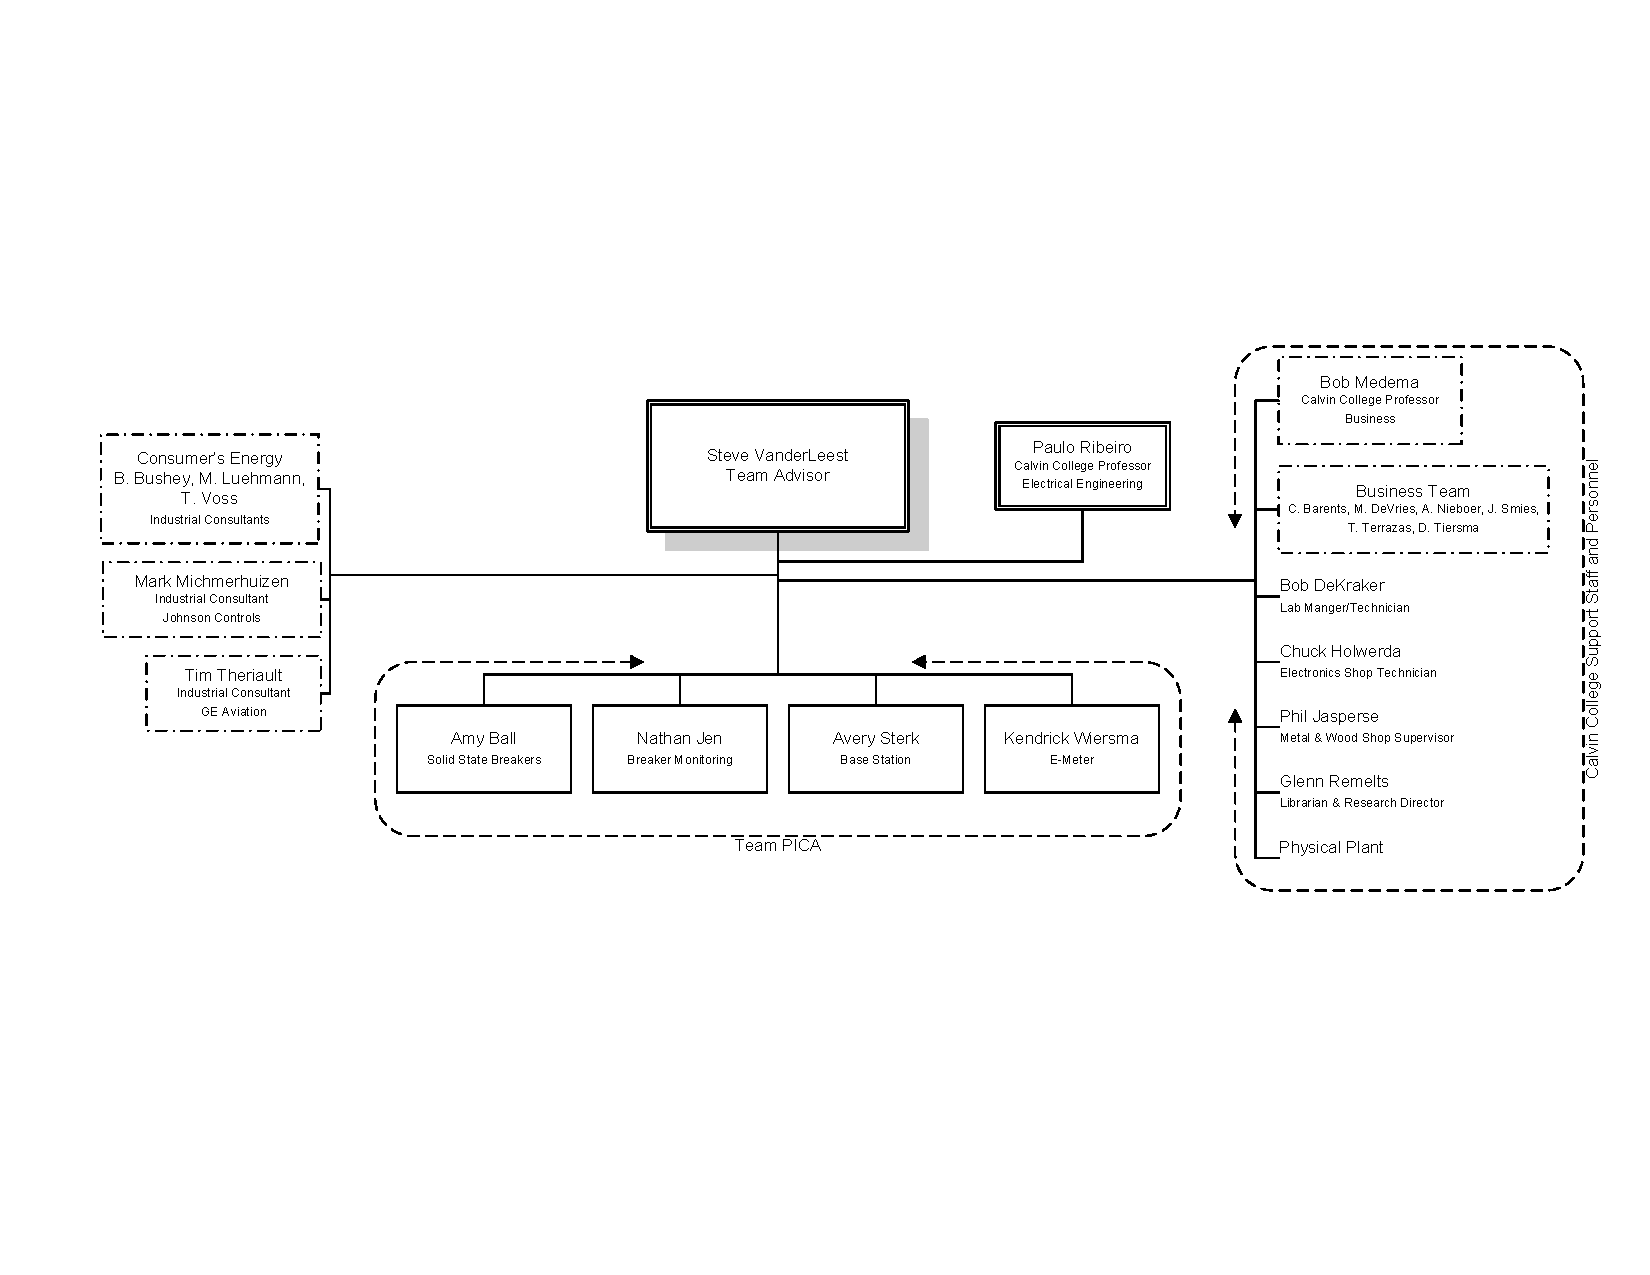
\includegraphics[width=6.5in]{figures/TeamOrgChart}
\caption{Team PICA Organizational chart.}
\label{fig:orgchart}
\end{center}
\end{figure}

\subsection{Team Responsibilities}
\subsubsection{Amy}
Amy, along with Nathan, makes up the hardware part of the team. They are in charge making decisions regarding hardware-specific sections of the project. Amy is also in charge of the Breaker sub-system of the project. She has the most complete understanding of their functions and specific requirements, she may delegate sub-sections to other team members, but she will have a good grasp of how they fit into the larger system. A sub-system of the Breakers is the monitoring section, which the team delegates to Nathan. Nathan and Amy will be working together closely with the full sub-system of the solid-state breakers.

\subsubsection{Nathan}
Nathan is co-leader with Kendrick. They are in charge of scheduling and assigning tasks, scheduling meetings, keeping team on time, on task, and will answer project questions. Nathan, along with Amy, makes up the hardware part of the team. They are in charge making decisions regarding hardware-specific sections of the project. Nathan is also in charge of helping integrate the sub-sections into the whole system, which includes having a detailed, basic understanding of each sub-system, and knowing how each relates to the overall requirements and goals. Nathan is also in charge of the monitoring section of the solid-state breakers.

\subsubsection{Avery}
Avery is in charge of the Base Station section of the project. He has the most complete understanding of it's function and specific requirements. He may delegate sub-sections to other team members, but he will have a good grasp of how they fit into the larger system. He, along with Kendrick, makes up the software part of the team; they make decisions regarding software-heavy sections of the project.

\subsubsection{Kendrick}
Kendrick is in charge of the E-Panel section of the project. He has the most complete understanding of it's function and specific requirements. He may delegate sub-sections to other team members, but he will have a good grasp of how they fit into the larger system. He is also co-leader with Nathan and they will share duties as necessary. He, along with Avery, makes up the software part of the team; they make decisions regarding software-heavy sections of the project.

\subsection{Schedule}
In order to complete the project within the established deadlines, the design team established a schedule and task-oriented deadlines to supplement the larger senior design program-established deadlines. In doing so, the design team selected to address the subsystems individually. The design team will first focus on the solid-state circuit breakers and circuit-monitoring devices, which they hope to complete by the end of the fall semester. The other two subsystems, the base station and the main smart meter, will gain focus in the second semester. Table \ref{Task_list.tex} shows a list of major milestones for the project with the estimated date of completion for each. The chart also shows the number of hours estimated needed for each task and any dependencies. Items in bold indicate tasks scheduled for completion by the current date and labor totals are shown in the bottom right. 

{
\small
\begin{longtable}[c]{|>{\raggedright}b{2in}|>{\raggedright}b{1in}|>{\raggedright}b{1in}|b{0.75in}|b{1in}|}
\caption{Task lists\label{Task_list.tex}}\\
\hline
\rowcolor{lightgray}
Milestone & Estimated Completion & Dependence & Estimated Labor &  \\
\hline
\endfirsthead
\caption[]{Continued from previous page}\\

\hline
\rowcolor{lightgray}
Milestone & Estimated Completion & Dependence & Estimated Labor &  \\
\hline
\endhead
\multicolumn{5}{r}{{Continued on next page}} \\
\endfoot

\endlastfoot
Project scope and functionality determined & Oct 25, 2010                                & none                      & 40  &              \\\hline
Project goals and requirements set         & Nov 16, 2010                                & Scope and functionality   & 60  &              \\\hline
Design criteria determined                 & Nov 19, 2010                                & Goals and requirements    & 15  &              \\\hline
Preliminary breaker design set             & Nov 23, 2010                                & Criteria                  & 50  &              \\\hline
Preliminary e-meter design set             & Feb 2, 2010                                 & Criteria                  & 50  &              \\\hline
Preliminary base station design set        & Mar 6, 2010                                 & Criteria                  & 50  &              \\\hline
Breaker prototyped and tested              & Dec 1, 2010                                 & Design set                & 30  &              \\\hline
E-meter prototyped and tested              & Feb 13, 2010                                & Design set                & 30  &              \\\hline
Base station prototyped and tested         & Mar 19, 2010                                & Design set                & 30  &              \\\hline
Full system integration                    & Apr 17, 2010                                & All subsystems prototyped & 40  &              \\\hline
PPFS turned in                             & Dec 7, 2010                                 & Criteria                  & 130 &              \\\hline
Project presented                          & May 16, 2010                                & Prototyped                & 40  &              \\\hline
                                           &                                             &                           & 325 & 1st Semester \\\hline
                                           &                                             &                           & 240 & 2nd Semester \\\hline
                                           &                                             &                           & 565 & Total        \\\hline
\end{longtable}
}



While subsystems should be able to be completed independent of each other, the design team decided to address the circuit-by-circuit monitoring component of the project first because of its application to control systems. As members of the design team are taking a class in control systems during the fall semester, working on the breakers while also learning control theory seemed to create an advantageous symbiosis between working and learning. The control systems course also seeks to use aspects of the senior design project as learning experiences, so the motivation to combine the controls assignment and the breaker modules is twofold.

The design team has assembled its internal schedule into Gantt chart to show the deadlines of tasks and the linkages between different tasks. Despite having this planning tool and list of tasks, the actual flow and completion of work is frequently different from originally expected. This is partially due to unexpected emergence of assignments and deadlines for the design project itself, but other classes also contribute unforeseen and time-consuming work that impedes progress in the project. To deal with outside deadlines and work, the team tried to think of deadlines focus on work and deadlines to two or three weeks out. Team members were encouraged to think in general terms only about deadlines more than a couple weeks out to help keep focus on current progress. As the semester progresses, these emergent due-dates should decrease in number and severity, allowing the design team to devote more time to the project.

In order to complete the project, the team needs to accomplish a variety of tasks shown in the work breakdown structure below. Much of the early work includes a lot of paperwork outside of the actual design of the system. This includes determining exactly what problem the team is addressing and the requirements needed to solve it. Project goals and design criteria also make up some of the pre-design work. In industry, the customer would already have set many of these requirements, goals and criteria, so to make the project as `real-world-like' as possible, the team put these before the design stage of the project. To make the requirements and goals realistic, the team decided to meet with a variety of professionals in fields including marketing, business and engineering in addition to potential customers. 

Once the project goals, requirements and criteria are set, the team can begin some preliminary design. As another way to limit the project and keep it from getting out of control, the project scope needs to be determined early in the project. A big factor in setting the scope is making the system unique from products that solve similar problems. The first step the team would like to take is to determine the basic functionality of both systems and subsystems and set up functional block diagrams to show this. After the basic functions of each of the subsystems are determined, the team will explore various solutions through general research and trade studies. When the team has compiled a number of different solutions, they can start to eliminate possibilities based on criteria established earlier. To assist with this, the team will use design matrices and comparison tables as visual aids.

After narrowing down the possible solutions, the team will begin the design and implementation stage. Further criteria may include power efficiency, cost of building the system, and availability of components. As  design aspects apply to all subsystems, and since development of the subsystems will occur at different rates as mentioned earlier, the finalized designs will not finish simultaneously. Testing will occur after designing and building the various parts of the subsystems. The team decided that the breakers, breaker monitors, main system monitor and wireless communication should be the first parts of the system completed. Other parts that will require finalization and building include the upgrade mechanism, base station, display module and firmware. Each of the parts will require modifications based on the testing results. Modifications to each of the parts may be necessary based on the testing results, so this section may take multiple iterations before it is complete.

Assembly of the full system will follow the individual parts' completion, along with testing for a variety of things. Some specific things the team hopes to include in the testing are tests based on outside criteria, tests based on requirements set by the team and testing common possible failure points. As the team is working with a limited amount of time that may not allow for full testing of the system, some of the long term testing procedures including accelerated lifetime testing will be written up for later use outside of the class.

Communication will be critical to the success of the project, both during and after so the team aims to provide documentation of all design decisions and testing done throughout the year. As the customer will need to interact with the system effectively, the team hopes to provide a user manual as well. For the class, the team needs to present the project on a number of occasions and hopes to demonstrate their work to all groups associated with the project, including business groups, customers and technical professionals.


  %includes scheduling crap that Nate didn't want to deal with
\section{Plan of Operation}


\subsection{Legal form of ownership}
The business shall be formed as a limited liability company under the name "PICA, LLC."

\subsection{Company structure}

\begin{figure}[htbp]
 \begin{center}
  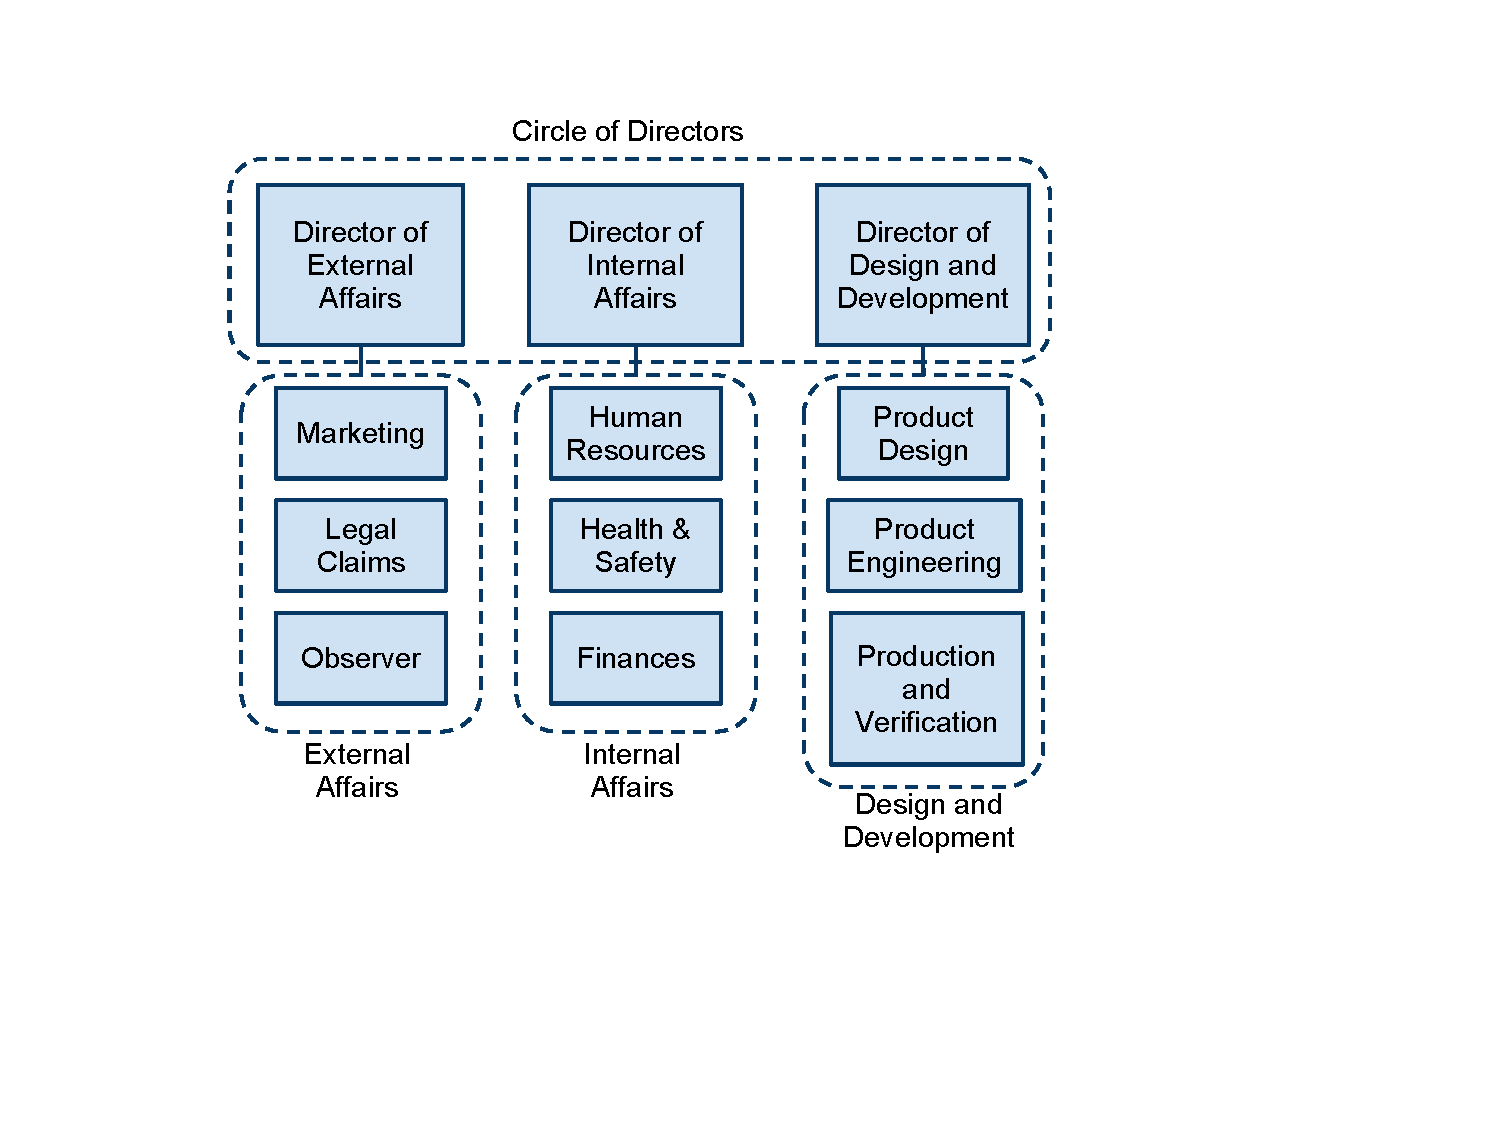
\includegraphics[trim=1.5in 1.75in 3in 0.75in,clip,width=0.6\textwidth]{figures/PICA_LLC_Org_Chart}
 \end{center}
 \caption{Proposed Organization Chart for PICA, LLC.}
 \label{fig:org-chart}
\end{figure}

\subsubsection{Select explanations of Figure \ref{fig:org-chart} }
The Internal Affairs directorate shall provide certain services to the other directorates and departmetns. For example, Internal Affairs includes the Human Resources division, but the other directorates will of course require the services of the HR division in order to hire new employees. Similarly, the finances division will provide budgeting information to the other divisions and directorates.

The other two directorates do not provide services to the other directorates. The one exception to this is the Observer function of the External Affairs directorate: its purpose is to monitor the business and legal climate in terms to demands and regulations, then inform the appropriate divisions. This could be spun off into its own directorate, but will likely not employ enough people to grant it a director and a direct voice in the Circle of Directors.

\subsection{Decision-making authority chain}
The final authority on a decision shall be vested in the Circle of Directors, but their authority shall not be required in every decision. The Circle of Directors shall have the exclusive power to make decisions regarding the direction of the business and the relationships between the directorates. Other issues may rise to the Circle if they cannot be resolved at a lower level or if the scope of the decision cannot be contained to one directorate. Otherwise, decisions that are limited in scope to any particular group or body shall be resolved within that body with the advice of the applicable Internal Affairs departments.



\subsection{Compensation/benefits package}
All employees shall be compensated fairly and in proportion to the scope of their decisions and actions. The company shall provide benefits packages including medical- prescription, vision, and dental plans. In addition, the company shall also provide a cafeteria and snacks for its employees to enjoy within moderation. The lowest Engineering position shall pay an annual salary of \$55,000, with up to 50\% increases in pay for each level of management ascended. Employees in other directorates will earn an annual salary of \$35,000, with a similar reward for ascending management. Employees shall receive raises in pay for distinguishing their work from that of their peers.



%\section{Financial Forecasts}
\subsection{E-Meter}
{
\small
\begin{longtable}[c]{|c|R|R|R|}
\caption{Pro-Forma Statement of Income\label{IncomeStatement.tex}}\\
\hline
\rowcolor{lightgray}
 & \mathrm{Year\ 1} & \mathrm{Year\ 2} & \mathrm{Year\ 3} \\\hline
\endfirsthead
\caption[]{Continued from previous page}\\

\hline
\rowcolor{lightgray}
 & \mathrm{Year\ 1} & \mathrm{Year\ 2} & \mathrm{Year\ 3} \\\hline
\endhead
\multicolumn{4}{r}{{Continued on next page}} \\
\endfoot

\endlastfoot
\hline
Sales revenue               & 190000000 & 238336000 & 266936320 \\\hline
Variable Cost of Goods Sold & 167245000 & 209792128 & 234967183 \\\hline
Fixed Cost of Goods Sold    & 1867500   & 2342592   & 2623703   \\\hline
Depreciation                & 2858      & 4898      & 3498      \\\hline
Gross Margin                & 20884642  & 26196382  & 29341936  \\\hline
Variable Operating Costs    & 16600000  & 20823040  & 23321805  \\
\hline
Fixed Operating Costs       & 31470     & 18621     & 13103     \\
\hline
Operating Income            & 4253172   & 5354721   & 6007028   \\
\hline
Interest Expense            & 30000     & 105000    & 204000    \\
\hline
Income Before Tax           & 4223172   & 5249721   & 5803028   \\
\hline
Income tax (40\%)            & 1689269   & 2099889   & 2321211   \\
\hline
Net Income After Tax        & 2533903   & 3149833   & 3481817   \\
\hline
\hline
\end{longtable}
}

{
\small
\begin{longtable}[c]{|c|R|R|R|}
\caption{Pro-Forma Statement of Cash Flow\label{CashFlow.textex}}\\
\hline
\rowcolor{lightgray}
 & \mathrm{Year\ 1} & \mathrm{Year\ 2} & \mathrm{Year\ 3} \\\hline
\endfirsthead
\caption[]{Continued from previous page}\\

\hline
\rowcolor{lightgray}
  & \mathrm{Year\ 1} & \mathrm{Year\ 2} & \mathrm{Year\ 3} \\\hline
 \endhead
\multicolumn{4}{r}{{Continued on next page}} \\
\endfoot

\endlastfoot
Beginning Cash Balance                & 0       & 4016761 & 9421492  \\
\hline
Net Income After Tax                  & 2533903 & 3149833 & 3481817  \\
\hline
Depreciation expense                  & 2858    & 4898    & 3498     \\
\hline
Invested Capital (Equity)             & 1000000 & 1500000 & 2000000  \\
\hline
Increase (decrease) in borrowed funds & 500000  & 750000  & 900000   \\
\hline
Equipment Purchases                   & -20000  & 0       & 0        \\
\hline
Ending Cash Balance                   & 4016761 & 9421492 & 15806807 \\
\hline
\hline
\end{longtable}
}

{
\small
\begin{longtable}[c]{|c|R|R|R|R|R|R|}
\caption{E-Meter Break Even Analysis\label{BreakEvenAnalysistex}}\\
\hline
\rowcolor{lightgray}
& \multicolumn{2}{|c|}{Year 1} &  \multicolumn{2}{c}{Year 2} &  \multicolumn{2}{|c|}{Year 3} \\\hline
\endfirsthead
\caption[]{Continued from previous page}\\

\hline
\rowcolor{lightgray}
 & \multicolumn{2}{|c|}{Year 1} &  \multicolumn{2}{c}{Year 2} &  \multicolumn{2}{|c|}{Year 3} \\\hline
 \endhead
\multicolumn{7}{r}{{Continued on next page}} \\
\endfoot

\endlastfoot

Sales revenue                        &           & 190000000    &           & 238336000 &           & 266936320 \\\hline
Less: Variable Costs:                &           &              &           &           &           &           \\\hline
Variable Cost of Goods Sold          & 167245000 &              & 209792128 &           & 234967183 &           \\\hline
Variable Operating Costs             & 16600000  &              & 20823040  &           & 23321805  &           \\\hline
Total Variable Costs                 &           & 183845000    &           & 230615168 &           & 258288988 \\\hline
Contribution Margin                  &           & 6155000      &           & 7720832   &           & 8647332   \\\hline
Less: Fixed Costs                    &           &              &           &           &           &           \\\hline
Fixed Cost of Goods Sold             & 1867500   &              & 2342592   &           & 2623703   &           \\\hline
Fixed Operating Costs                & 31470     &              & 18621     &           & 13103     &           \\\hline
Depreciation                         & 2858      &              & 4898      &           & 3498      &           \\\hline
Interest Expense                     & 30000     &              & 105000    &           & 204000    &           \\\hline
Total Fixed Costs                    &           & 1931828      &           & 2471111   &           & 2844304   \\
\hline
Income Before Tax                    &           & 4223172      &           & 5249721   &           & 5803028   \\\hline
\end{longtable}
}
{
\small
\begin{longtable}[c]{|c|R|R|R|}
\caption{E-Meter Break even sales volume\label{BreakEvenAnalysistex}}\\
\hline
\rowcolor{lightgray}
& \multicolumn{1}{|c|}{Year 1} &  \multicolumn{1}{c}{Year 2} &  \multicolumn{1}{|c|}{Year 3} \\\hline
\endfirsthead
\caption[]{Continued from previous page}\\

\hline
\rowcolor{lightgray}
 & \multicolumn{1}{|c|}{Year 1} &  \multicolumn{1}{c}{Year 2} &  \multicolumn{1}{|c|}{Year 3} \\\hline
 \endhead
\multicolumn{4}{r}{{Continued on next page}} \\
\endfoot

\endlastfoot

Total Fixed Costs                    & 1931828   & 2471111      & 2844304     \\\hline
Contribution Margin \%                & 3\%        & 3\%           & 3\%          \\\hline
Break Even Sales Volume              & 59634008  & 76281241     & 87801409   \\\hline
\end{longtable}
}
{
\small
\begin{longtable}[c]{|c|R|R|R|R|}
\caption{E-Meter Equipment and depreciation\label{BreakEvenAnalysistex}}\\
\hline
\rowcolor{lightgray}
& \mathrm{Equipment\ Purchases} & \multicolumn{1}{|c|}{Year 1} &  \multicolumn{1}{c}{Year 2} &  \multicolumn{1}{|c|}{Year 3} \\\hline
\endfirsthead
\caption[]{Continued from previous page}\\

\hline
\rowcolor{lightgray}
& \mathrm{Equipment\ Purchases} & \multicolumn{1}{|c|}{Year 1} &  \multicolumn{1}{c}{Year 2} &  \multicolumn{1}{|c|}{Year 3} \\\hline
 \endhead
\multicolumn{5}{r}{{Continued on next page}} \\
\endfoot

\endlastfoot

Equipment Purchases Year 1           & 20000     & 2858         & 4898      & 3498\\\hline
Equipment Purchases Year 2           & 0              &                    & 0            & 0 \\\hline
Equipment Purchases Year 3           & 0              &                    &                & 0 \\\hline
Annualized Total                                 &                 & 2858          & 4898      & 3498 \\\hline\hline
MACRS Rates (7-year recovery period) & 0.1429    & 0.2449       & 0.1749    &    \\\hline\hline
Interest Expense:                    &           &              &           &\\\hline
Annual interest rate on debt         & 12\%       &              &           & \\\hline
\end{longtable}
}

{
\small
\begin{longtable}[c]{|c|R|R|R|}
\caption{E-Meter Debt Balance\label{BreakEvenAnalysistex}}\\
\hline
\rowcolor{lightgray}
& \multicolumn{1}{|c|}{Year 1} &  \multicolumn{1}{c}{Year 2} &  \multicolumn{1}{|c|}{Year 3} \\\hline
\endfirsthead
\caption[]{Continued from previous page}\\

\hline
\rowcolor{lightgray}
 & \multicolumn{1}{|c|}{Year 1} &  \multicolumn{1}{c}{Year 2} &  \multicolumn{1}{|c|}{Year 3} \\\hline
 \endhead
\multicolumn{4}{r}{{Continued on next page}} \\
\endfoot

\endlastfoot
Average debt balance                 & 250000    & 875000       & 1700000\\
\hline
Interest expense                     & 30000     & 105000       & 204000\\
\hline
\end{longtable}
}


\subsection{Base Station}

{
\small
\begin{longtable}[c]{|c|R|R|R|}
\caption{Base Station Income Statement\label{IncomeStatement.tex}}\\
\hline
\rowcolor{lightgray}
 & \mathrm{Year\ 1} & \mathrm{Year\ 2} & \mathrm{Year\ 3} \\\hline
\endfirsthead
\caption[]{Continued from previous page}\\

\hline
\rowcolor{lightgray}
 & \mathrm{Year\ 1} & \mathrm{Year\ 2} & \mathrm{Year\ 3} \\\hline
\endhead
\multicolumn{4}{r}{{Continued on next page}} \\
\endfoot

\endlastfoot
Sales revenue               & 10000000  & 12544000         & 14049280         \\
\hline
Variable Cost of Goods Sold & 6432000   & 8068300.80        & 9036496.89      \\
\hline
Fixed Cost of Goods Sold    & 48000     & 60211.20          & 67436.54        \\
\hline
Depreciation                & 2858      & 4898             & 3498             \\
\hline
Gross Margin                & 3517142   & 4410590          & 4941848.56       \\
\hline
Variable Operating Costs    & 768000    & 963379.20         & 1078984.70      \\
\hline
Fixed Operating Costs       & 6470      & 74832.06 & 52655.65 \\
\hline
Operating Income            & 2742672   & 3372378.73 & 3810208.20 \\
\hline
Interest Expense            & 15000     & 48000            & 84000            \\
\hline
Income Before Tax           & 2727672   & 3324378.74 & 3726208.20 \\
\hline
Income tax (40\%)            & 1091068.80 & 1329751.49 & 1490483.28 \\
\hline
Net Income After Tax        & 1636603.20 & 1994627.24 & 2235724.92 \\
\hline
\end{longtable}
}

{
\small
\begin{longtable}[c]{|c|R|R|R|}
\caption{Base Station Cash Flow\label{CashFlow.tex}}\\
\hline
\rowcolor{lightgray}
 & \mathrm{Year\ 1} & \mathrm{Year\ 2} & \mathrm{Year\ 3} \\\hline
\endfirsthead
\caption[]{Continued from previous page}\\

\hline
\rowcolor{lightgray}
 & \mathrm{Year\ 1} & \mathrm{Year\ 2} & \mathrm{Year\ 3} \\\hline
\endhead
\multicolumn{4}{r}{{Continued on next page}} \\
\endfoot

\endlastfoot
                                      &           &                  &                  \\
\hline
Beginning Cash Balance                & 0         & 2369461.20        & 5268986.44 \\
\hline
Net Income After Tax                  & 1636603.20 & 1994627.24 & 2235724.92 \\
\hline
Depreciation expense                  & 2858      & 4898             & 3498             \\
\hline
Invested Capital (Equity)             & 500000    & 600000           & 650000           \\
\hline
Increase (decrease) in borrowed funds & 250000    & 300000           & 300000           \\
\hline
Equipment Purchases                   & -20000    & 0                & 0                \\
\hline
Ending Cash Balance                   & 2369461.20 & 5268986.44 & 8458209.36 \\
\hline
\hline
\end{longtable}
}

{
\small
\begin{longtable}[c]{|c|R|R|R|R|R|R|}
\caption{Base Station Break Even Analysis\label{BreakEvenAnalysis.tex}}\\
\hline
\rowcolor{lightgray}
& \multicolumn{2}{|c|}{Year 1} &  \multicolumn{2}{c}{Year 2} &  \multicolumn{2}{|c|}{Year 3} \\\hline
\endfirsthead
\caption[]{Continued from previous page}\\

\hline
\rowcolor{lightgray}
& \multicolumn{2}{|c|}{Year 1} &  \multicolumn{2}{c}{Year 2} &  \multicolumn{2}{|c|}{Year 3} \\\hline
\endhead
\multicolumn{7}{r}{{Continued on next page}} \\
\endfoot

\endlastfoot
Sales revenue                        &                     & 10000000.00      &                  & 12544000.00 &            & 14049280.00 \\
\hline
Less: Variable Costs:                &                     &                  &                  &             &            &             \\
\hline
Variable Cost of Goods Sold          & 6432000.00          &                  & 8068300.80       &             & 9036496.90 &             \\
\hline
Variable Operating Costs             & 768000.00           &                  & 963379.20        &             & 1078984.70 &             \\
\hline
Total Variable Costs                 &                     & 7200000.00       &                  & 9031680.00  &            & 10115481.60 \\
\hline
Contribution Margin                  &                     & 2800000.00       &                  & 3512320.00  &            & 3933798.40  \\
\hline
Less: Fixed Costs                    &                     &                  &                  &             &            &             \\
\hline
Fixed Cost of Goods Sold             & 48000.00            &                  & 60211.20         &             & 67436.54   &             \\
\hline
Fixed Operating Costs                & 6470.00             &                  & 74832.06         &             & 52655.66   &             \\
\hline
Depreciation                         & 2858.00             &                  & 4898.00          &             & 3498.00    &             \\
\hline
Interest Expense                     & 15000.00            &                  & 48000.00         &             & 84000.00   &             \\
\hline
Total Fixed Costs                    &                     & 72328.00         &                  & 187941.26   &            & 207590.20   \\
\hline
Income Before Tax                    &                     & 2727672.00       &                  & 3324378.74  &            & 3726208.20  \\\hline
\end{longtable}
}
{
\small
\begin{longtable}[c]{|c|R|R|R|}
\caption{Base Station Break even sales volume\label{BreakEvenAnalysistex}}\\
\hline
\rowcolor{lightgray}
& \multicolumn{1}{|c|}{Year 1} &  \multicolumn{1}{c}{Year 2} &  \multicolumn{1}{|c|}{Year 3} \\\hline
\endfirsthead
\caption[]{Continued from previous page}\\

\hline
\rowcolor{lightgray}
 & \multicolumn{1}{|c|}{Year 1} &  \multicolumn{1}{c}{Year 2} &  \multicolumn{1}{|c|}{Year 3} \\\hline
 \endhead
\multicolumn{4}{r}{{Continued on next page}} \\
\endfoot

\endlastfoot

Total Fixed Costs                    & 72328               & 187941.26 & 207590.19 \\
\hline
Contribution Margin \%                & 28\%                 & 28\%              & 28\%                     \\\hline
Break Even Sales Volume              & 258314.29           & 671218.79        & 741393.57                \\\hline
\end{longtable}
}
{
\small
\begin{longtable}[c]{|c|R|R|R|R|}
\caption{Base Station Equipment and depreciation\label{BreakEvenAnalysistex}}\\
\hline
\rowcolor{lightgray}
& \mathrm{Equipment\ Purchases} & \multicolumn{1}{|c|}{Year 1} &  \multicolumn{1}{c}{Year 2} &  \multicolumn{1}{|c|}{Year 3} \\\hline
\endfirsthead
\caption[]{Continued from previous page}\\

\hline
\rowcolor{lightgray}
& \mathrm{Equipment\ Purchases} & \multicolumn{1}{|c|}{Year 1} &  \multicolumn{1}{c}{Year 2} &  \multicolumn{1}{|c|}{Year 3} \\\hline
 \endhead
\multicolumn{5}{r}{{Continued on next page}} \\
\endfoot

\endlastfoot

Equipment Purchases Year 1           & 20000               & 2858             & 4898             & 3498 \\\hline
Equipment Purchases Year 2           & 0                   &                  & 0                & 0\\\hline
Equipment Purchases Year 3           & 0                   &                  &                  & 0      \\\hline
Annualized Totals                               &                     & 2858             & 4898             & 3498                 \\\hline
MACRS Rates (7-year recovery period) & 0.1429              & 0.2449           & 0.1749           &             \\\hline
Interest Expense:                    &                     &                  &                  &             \\\hline
Annual interest rate on debt         & 12\%                 &                  &                  &                   \\\hline
\end{longtable}
}

{
\small
\begin{longtable}[c]{|c|R|R|R|}
\caption{Base Station Debt Balance\label{BreakEvenAnalysistex}}\\
\hline
\rowcolor{lightgray}
& \multicolumn{1}{|c|}{Year 1} &  \multicolumn{1}{c}{Year 2} &  \multicolumn{1}{|c|}{Year 3} \\\hline
\endfirsthead
\caption[]{Continued from previous page}\\

\hline
\rowcolor{lightgray}
 & \multicolumn{1}{|c|}{Year 1} &  \multicolumn{1}{c}{Year 2} &  \multicolumn{1}{|c|}{Year 3} \\\hline
 \endhead
\multicolumn{4}{r}{{Continued on next page}} \\
\endfoot

\endlastfoot
Average debt balance                 & 125000              & 400000           & 700000           \\
\hline
Interest expense                     & 15000               & 48000            & 84000                  \\
\hline

\end{longtable}
}


\subsection{Solid State Breaker}

{
\small
\begin{longtable}[c]{|c|R|R|R|}
\caption{Breakers Income Statement\label{IncomeStatement.tex}}\\
\hline
\rowcolor{lightgray}
 & \mathrm{Year\ 1} & \mathrm{Year\ 2} & \mathrm{Year\ 3} \\\hline
\endfirsthead
\caption[]{Continued from previous page}\\

\hline
\rowcolor{lightgray}
 & \mathrm{Year\ 1} & \mathrm{Year\ 2} & \mathrm{Year\ 3} \\\hline
\endhead
\multicolumn{4}{r}{{Continued on next page}} \\
\endfoot

\endlastfoot
Sales revenue               & 90000000.00 & 112896000.00 & 126443520.00 \\\hline
Variable Cost of Goods Sold & 57600000.00 & 72253440.00  & 80923852.80  \\\hline
Fixed Cost of Goods Sold    & 2400000.00  & 3010560.00   & 3371827.20   \\\hline
Depreciation                & 2858.00     & 4898.00      & 3498.00      \\\hline
Gross Margin                & 29997142.00 & 37627102.00  & 42144342.00  \\\hline
Variable Operating Costs    & 25368000.00 & 31821619.20  & 35640213.50  \\\hline
Fixed Operating Costs       & 5000.00     & 2958.49      & 2081.74      \\\hline
Operating Income            & 4624142.00  & 5802524.31   & 6502046.75   \\\hline
Interest Expense            & 120000.00   & 360000.00    & 600000.00    \\\hline
Income Before Tax           & 4504142.00  & 5442524.31   & 5902046.75   \\\hline
Income tax (40\%)            & 1801656.80  & 2177009.72   & 2360818.70   \\\hline
Net Income After Tax        & 2702485.20  & 3265514.59   & 3541228.05   \\\hline
\end{longtable}
}

{
\small
\begin{longtable}[c]{|c|R|R|R|}
\caption{Base Station Cash Flow\label{CashFlow.tex}}\\
\hline
\rowcolor{lightgray}
 & \mathrm{Year\ 1} & \mathrm{Year\ 2} & \mathrm{Year\ 3} \\\hline
\endfirsthead
\caption[]{Continued from previous page}\\

\hline
\rowcolor{lightgray}
 & \mathrm{Year\ 1} & \mathrm{Year\ 2} & \mathrm{Year\ 3} \\\hline
\endhead
\multicolumn{4}{r}{{Continued on next page}} \\
\endfoot

\endlastfoot
                                      &            &             &             \\
\hline
Beginning Cash Balance                & 0.00       & 6685343.20  & 14455755.79 \\
\hline
Net Income After Tax                  & 2702485.20 & 3265514.59  & 3541228.05  \\
\hline
Depreciation expense                  & 2858.00    & 4898.00     & 3498.00     \\
\hline
Invested Capital (Equity)             & 2000000.00 & 2500000.00  & 3000000.00  \\
\hline
Increase (decrease) in borrowed funds & 2000000.00 & 2000000.00  & 2000000.00  \\
\hline
Equipment Purchases                   & -20000.00  & 0.00        & 0.00        \\
\hline
Ending Cash Balance                   & 6685343.20 & 14455755.79 & 23000481.84 \\
\hline
\hline
\end{longtable}
}

{
\small
\begin{longtable}[c]{|c|R|R|R|R|R|R|}
\caption{default\label{BreakEvenAnalysis.tex}}\\
\hline
\rowcolor{lightgray}
& \multicolumn{2}{|c|}{Year 1} &  \multicolumn{2}{c}{Year 2} &  \multicolumn{2}{|c|}{Year 3} \\\hline
\endfirsthead
\caption[]{Continued from previous page}\\

\hline
\rowcolor{lightgray}
& \multicolumn{2}{|c|}{Year 1} &  \multicolumn{2}{c}{Year 2} &  \multicolumn{2}{|c|}{Year 3} \\\hline
\endhead
\multicolumn{7}{r}{{Continued on next page}} \\
\endfoot

\endlastfoot
Sales revenue                        &             & 90000000.00  &             & 112896000.00 &             & 126443520.00 \\
\hline
Less: Variable Costs:                &             &              &             &              &             &              \\
\hline
Variable Cost of Goods Sold          & 57600000.00 &              & 72253440.00 &              & 80923852.80 &              \\
\hline
Variable Operating Costs             & 25368000.00 &              & 31821619.20 &              & 35640213.50 &              \\
\hline
Total Variable Costs                 &             & 82968000.00  &             & 104075059.20 &             & 116564066.30 \\
\hline
Contribution Margin                  &             & 7032000.00   &             & 8820940.80   &             & 9879453.70   \\
\hline
Less: Fixed Costs                    &             &              &             &              &             &              \\
\hline
Fixed Cost of Goods Sold             & 2400000.00  &              & 3010560.00  &              & 3371827.20  &              \\
\hline
Fixed Operating Costs                & 5000.00     &              & 2958.49     &              & 2081.74     &              \\
\hline
Depreciation                         & 2858.00     &              & 4898.00     &              & 3498.00     &              \\
\hline
Interest Expense                     & 120000.00   &              & 360000.00   &              & 600000.00   &              \\
\hline
Total Fixed Costs                    &             & 2527858.00   &             & 3378416.49   &             & 3977406.94   \\
\hline
Income Before Tax                    &             & 4504142.00   &             & 5442524.31   &             & 5902046.75   \\
\hline
\end{longtable}
}
{
\small
\begin{longtable}[c]{|c|R|R|R|}
\caption{Breaker Break even sales volume\label{BreakEvenAnalysistex}}\\
\hline
\rowcolor{lightgray}
& \multicolumn{1}{|c|}{Year 1} &  \multicolumn{1}{c}{Year 2} &  \multicolumn{1}{|c|}{Year 3} \\\hline
\endfirsthead
\caption[]{Continued from previous page}\\

\hline
\rowcolor{lightgray}
 & \multicolumn{1}{|c|}{Year 1} &  \multicolumn{1}{c}{Year 2} &  \multicolumn{1}{|c|}{Year 3} \\\hline
 \endhead
\multicolumn{4}{r}{{Continued on next page}} \\
\endfoot

\endlastfoot

Total Fixed Costs                    & 2527858.00  & 3378416.49   & 3977406.94            \\
\hline
Contribution Margin\%                & 7.81\%       & 7.81\%        & 7.81\%                  \\
\hline
Break Even Sales Volume              & 32353131.40 & 43239118.91  & 50905378.99            \\
\hline
\end{longtable}
}
{
\small
\begin{longtable}[c]{|c|R|R|R|R|}
\caption{Breaker Equipment and depreciation\label{BreakEvenAnalysistex}}\\
\hline
\rowcolor{lightgray}
& \mathrm{Equipment\ Purchases} & \multicolumn{1}{|c|}{Year 1} &  \multicolumn{1}{c}{Year 2} &  \multicolumn{1}{|c|}{Year 3} \\\hline
\endfirsthead
\caption[]{Continued from previous page}\\

\hline
\rowcolor{lightgray}
& \mathrm{Equipment\ Purchases} & \multicolumn{1}{|c|}{Year 1} &  \multicolumn{1}{c}{Year 2} &  \multicolumn{1}{|c|}{Year 3} \\\hline
 \endhead
\multicolumn{5}{r}{{Continued on next page}} \\
\endfoot

\endlastfoot
Equipment Purchases Year 1           & 20000       & 2858         & 4898        & 3498                   \\
\hline
Equipment Purchases Year 2           & 0           &              & 0           & 0              \\
\hline
Equipment Purchases Year 3           & 0           &              &             & 0                   \\
\hline
Annualized Total                     &             & 2858         & 4898        & 3498                  \\
\hline
MACRS Rates (7-year recovery period) & 0.1429      & 0.2449       & 0.1749      &             \\\hline
Interest Expense:                    &             &              &             &                        \\\hline
Annual interest rate on debt         & 12\%         &              &             &                       \\\hline
\end{longtable}
}

{
\small
\begin{longtable}[c]{|c|R|R|R|}
\caption{Breaker Debt Balance\label{BreakEvenAnalysistex}}\\
\hline
\rowcolor{lightgray}
& \multicolumn{1}{|c|}{Year 1} &  \multicolumn{1}{c}{Year 2} &  \multicolumn{1}{|c|}{Year 3} \\\hline
\endfirsthead
\caption[]{Continued from previous page}\\

\hline
\rowcolor{lightgray}
 & \multicolumn{1}{|c|}{Year 1} &  \multicolumn{1}{c}{Year 2} &  \multicolumn{1}{|c|}{Year 3} \\\hline
 \endhead
\multicolumn{4}{r}{{Continued on next page}} \\
\endfoot

\endlastfoot

Average debt balance                 & 1000000     & 3000000      & 5000000             \\
\hline
Interest expense                     & 120000      & 360000       & 600000                 \\
\hline
\end{longtable}
}

\newpage  % old section
{
\small
\begin{longtable}[c]{|c|c|r|c|c|c|c|r|}
\caption{Ten-Year Financial Forecast\label{ten_year_forecast.tex}}\\
\hline
\rowcolor{lightgray}
Year & Growth & Units Sold & Parts Cost & Other Cost & Income & Balance & Running Total \\ \hline\hline
\hline
\endfirsthead

\caption[]{Continued from previous page}\\
\hline
\rowcolor{lightgray}
 Year & Growth & Units Sold & Parts Cost & Other Cost & Income & Balance & Running Total \\ \hline\hline
\hline
\endhead

\multicolumn{8}{r}{{Continued on next page}} \\
\endfoot

\endlastfoot


1 & -- & 166000 & 56000000 & 242000 & 66000000 & 10283000 & 10283000 \\
2 & +2\% & 169000 & 57000000 & 149000 & 68000000 & 10587000 & 20870000 \\
3 & +2\% & 173000 & 58000000 & 149000 & 69000000 & 10801000 & 31671000 \\
4 & +5\% & 181000 & 61000000 & 149000 & 73000000 & 11349000 & 43020000 \\
5 & +2\% & 185000 & 62000000 & 149000 & 74000000 & 11579000 & 54599000 \\
6 & -10\% & 166000 & 56000000 & 149000 & 67000000 & 10406000 & 65005000 \\
7 & -10\% & 150000 & 50000000 & 149000 & 60000000 & 9350000 & 74355000 \\
8 & -12\% & 132000 & 44000000 & 149000 & 53000000 & 8210000 & 82565000 \\
9 & -12\% & 116000 & 39000000 & 149000 & 46000000 & 7207000 & 89772000 \\
10 & -15\% & 99000 & 33000000 & 149000 & 39000000 & 6104000 & 95876000 \\
\hline
\end{longtable}
} % new section


\section{Loan or Investment Proposal}

\subsection{Amount Requested -- Equity and/or Debt}
%3.5M\$
In order to successfully enter the smart metering market, PICA LLC feels that they will require \$290 million in assets. In order to have all these assets, we plan on using a 60-40 split for debt and equity. Thus, our debt-equity structure for startup becomes \$174 million in debt and \$116 million in equity. We hope to raise the \$116 million through personal donations from venture capitalists while the remainder of the cash supply comes from a business loan.

\subsection{Purpose and Uses of Funds}
We plan to initially contract for the fabrication of the circuit boards until we gain enough operating capital to move production in-house. Our startup costs represent initial cost of parts to begin production and salary for our employees during the first year. Until our business proves to be successful we plan on renting office and warehouse space for the first year. After the first year, assuming financial success, we hope to build our own warehouse to store completed systems before shipment to retailers.

\subsection{Repayment and Cash Out Schedule}
By year 5 of business, PICA LLC forecasts enough financial success to being repaying our venture capitalists. The return on investment for these venture capitalists, assuming economic success will be 8-10\% of the initial investment.

\subsection{Timetable for Implementing and Launching a Business}
PICA LLC projects a 6-month timeframe for starting the business. During these 6-months, PICA LLC intends to finish and prove the initial prototype and get all necessary contracts in place for office space, warehouse storage, shipping, and production facilities. After these are in place, PICA LLC projects that by the end of year 1, they will be shipping completed products to retail locations.


%\include{acknowledgements}
%\include{conclusions}
\bibliographystyle{IEEEtran}
\bibliography{bibliography}


\begin{appendix}
%\begin{table}[htdp]
%\caption{default}
\section{Acronyms}
\begin{acronym}[TDMA]
\acro{AC}{Alternating Current}
\acro{AD}{Analog Devices}
\acro{ADC}{Analog-to-Digital Converter}
\acro{AES}{Advanced Encryption Standard}
\acro{AMR}{Automated Meter Reading}
\acro{ANSI}{American National Standards Institute}
\acro{CAD}{Computer Aided Design}
\acro{CDMA}{Code Devision Multiple Access}
\acro{CF}{Compact Flash}
\acro{DC}{Direct Current}
\acro{DHCP}{Dynamic Host Configuration Protocol}
\acro{DOE}{United States Department of Energy}
\acro{EEPROM}{Electronically Erasable Programable Read Only Memory}
\acro{ESP}{Electronic Signal Processing}
\acro{EM}{electromagnetic}
\acro{FCC}{Federal Communications Commission}
\acro{FET}{Field-Effect Transistors}
\acro{FPGA}{Field Programable Gate Array}
\acro{GPL}{GNU General Public License}
\acro{HTTP}{Hypertext Transfer Protocol}
\acro{IC}{Integrated Circuit}
\acro{IEC}{International Electrotechnical Commision}
\acro{IEEE}{International Electrical and Electronics Engineers}
\acro{JCI}{Johnson Controls, Inc.}
\acro{LAN}{Local Area Network}
\acro{LCD}{Liquid Crystal Display}
\acro{LED}{Light Emitting Diode}
\acro{MCU}{Master Control Unit}
\acro{MSRP}{Manufacturer Suggested Retail Price}
\acro{NEMA}{National Electrical Manufacturers Association}
\acro{NIC}{Network Interface Card}
\acro{NILM}{Non-intrusive Load Monitoring}
\acro{NPC}{National Power Corporation}
\acro{NTP}{Network Time Protocol}
\acro{OS}{Operating System}
\acro{PC}{Personal Computer}
\acro{RAM}{Random-Access Memory}
\acro{RFID}{Radio Frequency Identification Device}
\acro{RMS}{Root Mean Square}
\acro{SD}{Secure Digital}
\acro{SoC}{System on a Chip}
\acro{SPI}{Serial Peripheral Bus}
\acro{TI}{Texas Instruments}
\acro{UL}{Underwriters Laboratories}
\end{acronym}
%\label{default}
%\end{table}%

%\section{Team Information}

Team 01, Team PICA seen in figure \ref{fig:teamphoto} consists of four engineers in Calvin College's Electrical and Computer Engineering concentration: Amy Ball, Nathan Jen, Avery Sterk, and Kendrick Wiersma.

\begin{figure}[htbp]
\begin{center}
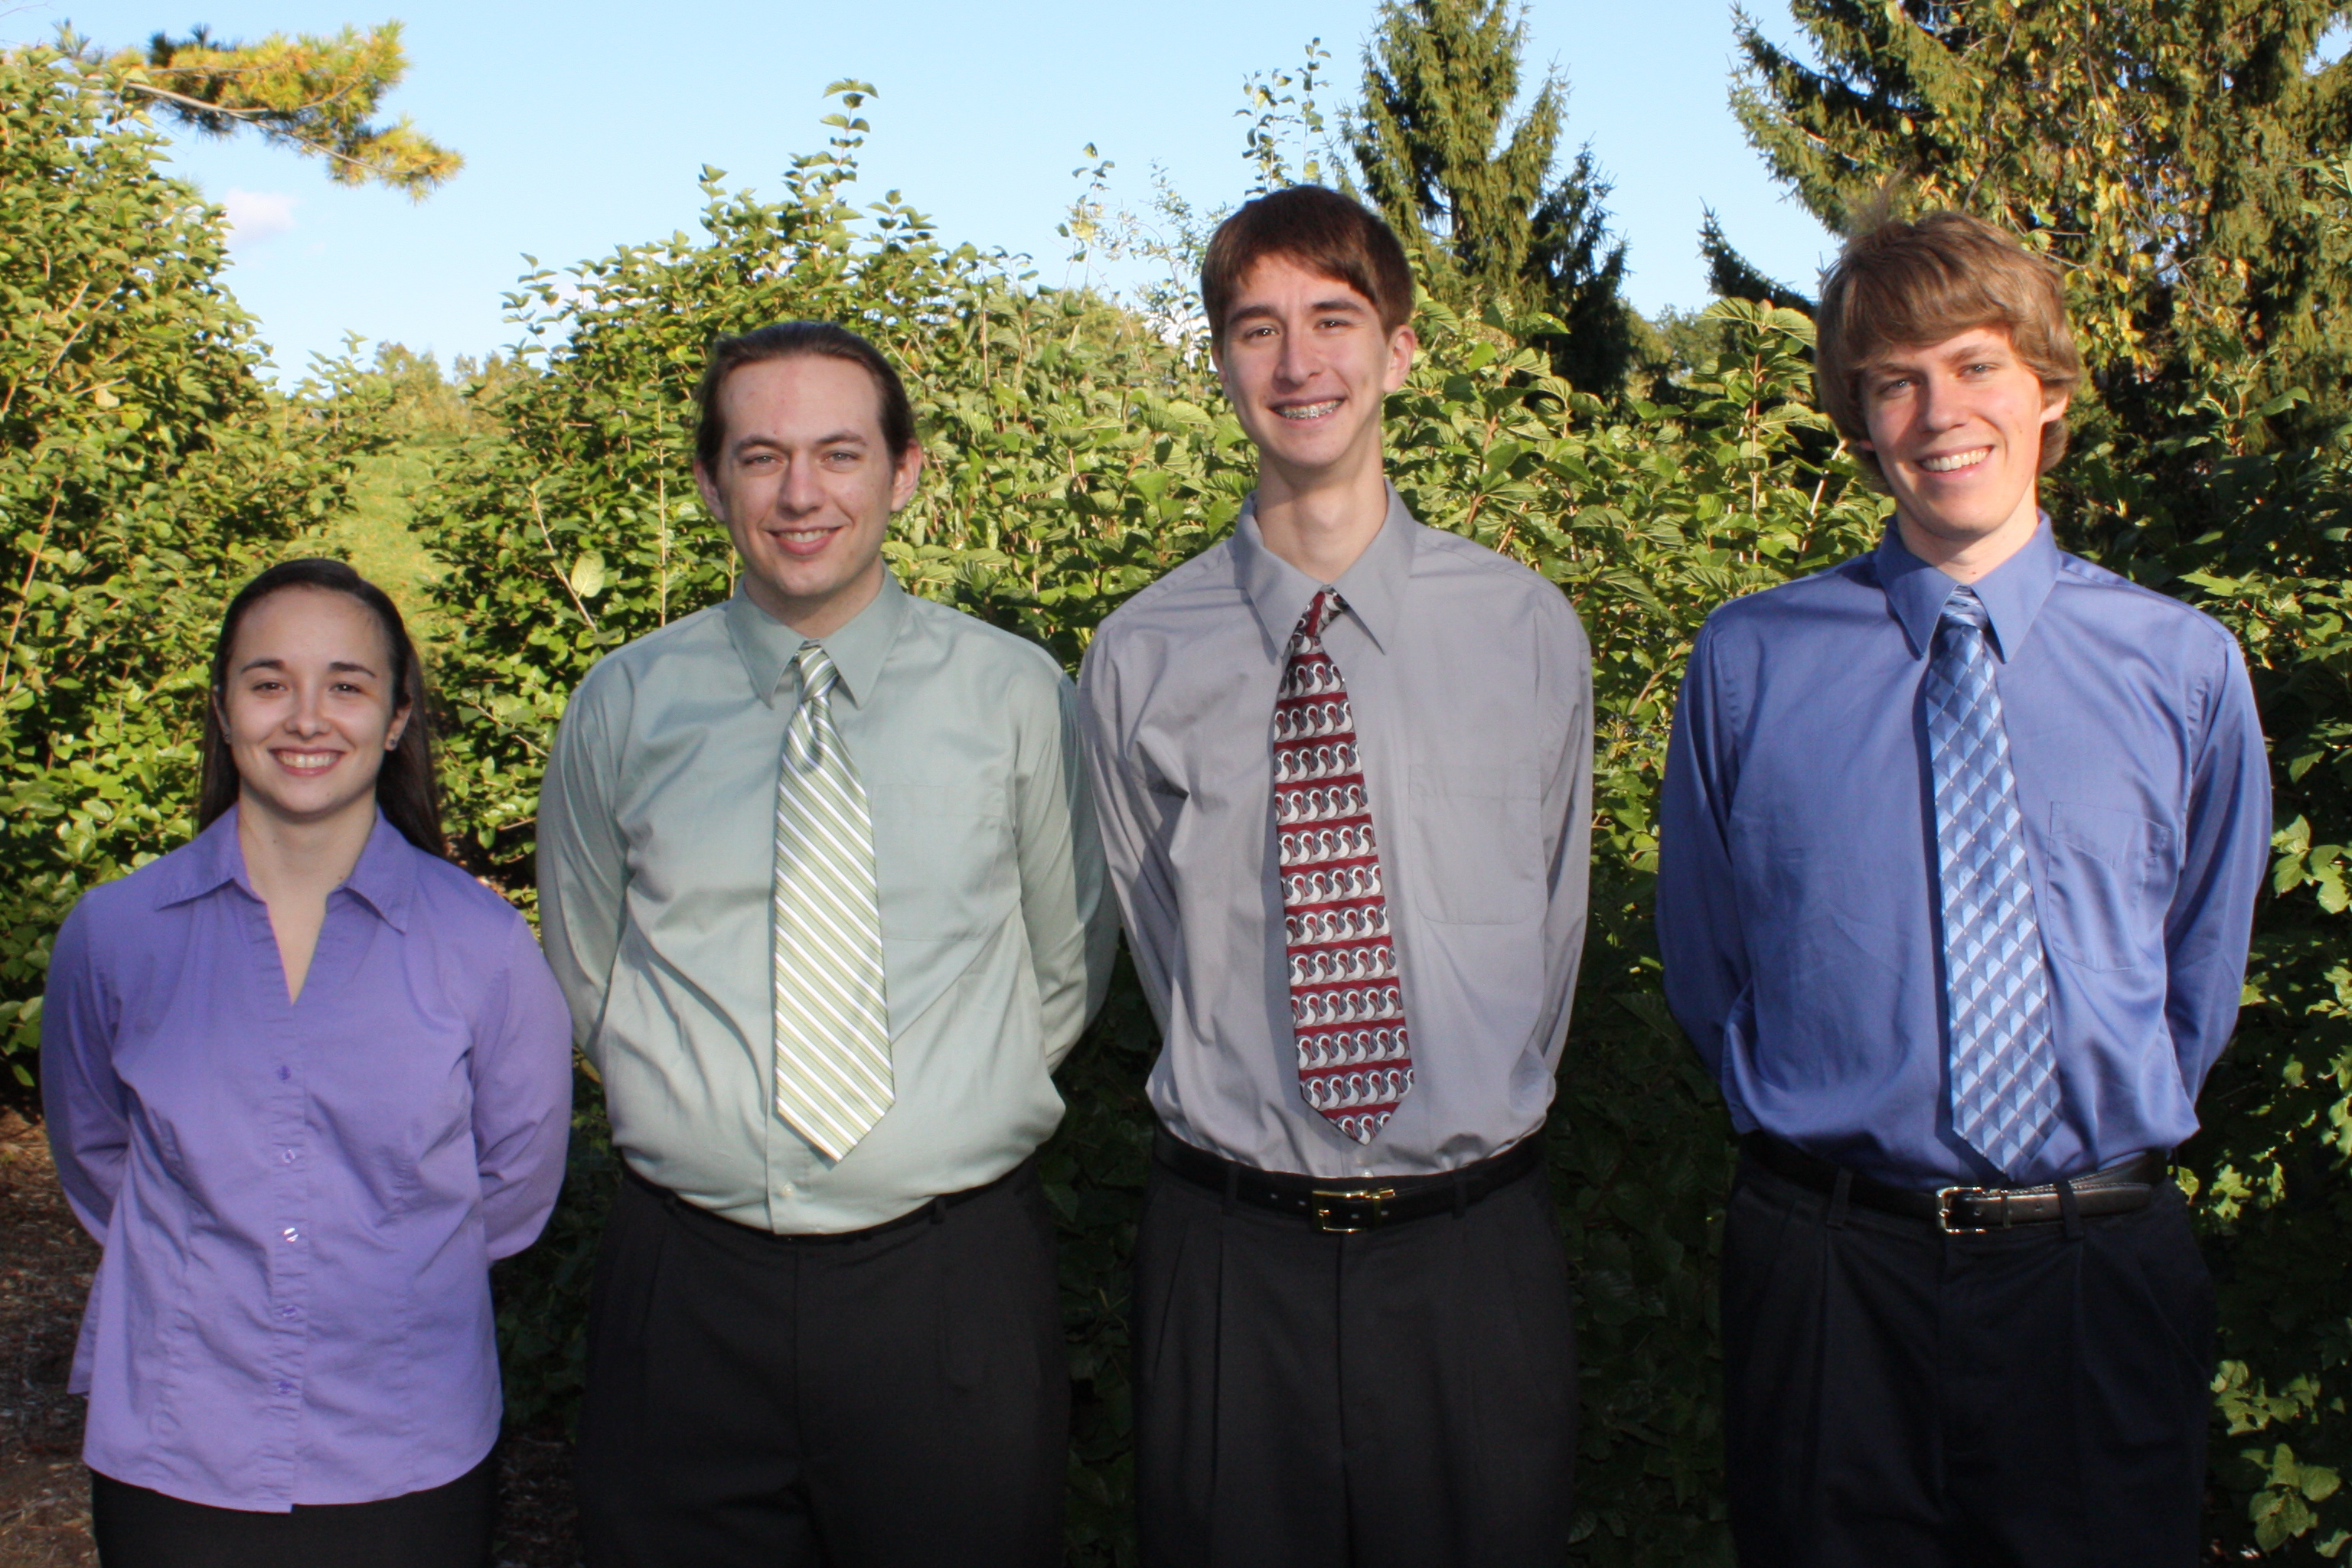
\includegraphics[width=6in]{figures/IMG_0865}
\caption{Team PICA, left to right: Amy Ball, Kendrick Wiersma, Nate Jen, and Avery Sterk.}
\label{fig:teamphoto}
\end{center}
\end{figure}

Amy works as an intern at Johnson Controls, where she works as part of the Systems Engineering Team. She brings good communication skills, circuit-building experience, and presentation skills to the project. Her section of the project is the solid-state breakers, especially working closely with much of the analog hardware involved with the project.

Kendrick works as an intern at Raytheon Missile Systems in the Electronics Center, where he performs embedded system design and verification. Kendrick hails from Tucson, Arizona where he was born and raised. He brings real-world project experience and experience working with embedded hardware and software to the team. Kendrick leads the development of the E-meter, which measures whole-building power consumption, reporting data to the power company and the PICA base station.

Nathan has worked at Amway on the production floor and has gained involvement with club leadership at Calvin College. He brings leadership experience and a good understanding of how smaller elements of a system fit together as a whole. His section of the project is the monitoring of individual circuits and some of the control logic for the breakers.

Avery worked as an intern at the SLAC National Accelerator Laboratory doing \ac{CAD} design. He brings varied experience with software design and implementation to the project. His section of the project is the base station, especially providing the primary user interface and designing embedded software.



%\section{Team Resumes}
%The following pages contain each team-member's resume.

%\includepdf[pages={1},pagecommand={},scale=.9]{resume/Ball_Amy}
%\includepdf[pages={1},pagecommand={},scale=.9]{resume/Wiersma_Kendrick}
%\includepdf[pages={1},pagecommand={},scale=.9]{resume/Jen_Nathan}
%\includepdf[pages={1},pagecommand={},scale=.9]{resume/Sterk_Avery} 
\end{appendix}

\end{spacing}
\end{document}

%%%%%%%%%%%%%%%%%%%%%%%%%%%%%%%%%%%%%%%%%%%%%%%%%%%%%%%%%%%%%
